\documentclass[13pt,a4paper]{article}
% A4, 12 pt, line spacing 1.25, margins 2.5 cm. Layout follows the I05 report.
% XeTeX path: T5 Latin Modern in this environment has no Vietnamese glyphs.
\usepackage{fontspec}
\setmainfont{LiberationSerif}[
  Path=/usr/share/fonts/truetype/liberation/,
  Extension=.ttf,
  UprightFont=*-Regular,
  BoldFont=*-Bold,
  ItalicFont=*-Italic,
  BoldItalicFont=*-BoldItalic]
\setsansfont{LiberationSans}[
  Path=/usr/share/fonts/truetype/liberation/,
  Extension=.ttf,
  UprightFont=*-Regular,
  BoldFont=*-Bold,
  ItalicFont=*-Italic,
  BoldItalicFont=*-BoldItalic]
\setmonofont{LiberationMono}[
  Path=/usr/share/fonts/truetype/liberation/,
  Extension=.ttf,
  UprightFont=*-Regular,
  BoldFont=*-Bold,
  ItalicFont=*-Italic,
  BoldItalicFont=*-BoldItalic,
  Scale=0.82]
\usepackage[vietnamese]{babel}
\usepackage{geometry}
\usepackage{setspace}
\usepackage{booktabs}
\setlength{\aboverulesep}{0pt}
\setlength{\belowrulesep}{0pt}
\setlength{\abovetopsep}{0pt}
\setlength{\belowbottomsep}{0pt}
\usepackage{tabularx}
\usepackage{etoolbox}
\pretocmd{\tabularx}{\ifvmode\noindent\fi}{}{}
\pretocmd{\section}{\clearpage}{}{}
\usepackage{array}
\usepackage{enumitem}
\usepackage{graphicx}
\usepackage{float}
\usepackage{pdflscape}
\usepackage{amsmath}
\usepackage{tikz}
\usetikzlibrary{arrows.meta,shapes.geometric}
\usepackage{verbatim}
\usepackage[hidelinks]{hyperref}
\newcommand{\figframe}[2]{%
  \begin{figure}[H]
  \centering
  \setlength{\fboxsep}{4pt}%
  \fbox{\begin{minipage}{0.92\textwidth}\centering #2\end{minipage}}%
  \caption{#1}
  \end{figure}%
}
\geometry{a4paper,margin=2.5cm}
\setstretch{1.25}
\newcolumntype{Y}{>{\raggedright\arraybackslash}X}
\setlength{\parskip}{0.4em}
\begin{document}

\begin{center}
{\Large TRƯỜNG ĐẠI HỌC PHENIKAA}\\[0.4em]
Khoa Điện-Điện tử\\[1em]
\vspace{1cm}
{\LARGE BÁO CÁO}\\[0.5em]
{\large Nén một mạng nơ-ron tích chập đã huấn luyện trên Fashion-MNIST\\ để triển khai bằng TensorFlow Lite}\\[0.6em]
\end{center}
\vspace{1.2cm}
\begin{tabularx}{\textwidth}{|>{\raggedright\arraybackslash}p{4.6cm}|Y|}
\hline
Học phần & TODO \\ \hline
Mã học phần & TODO \\ \hline
Tên bài & DL-10 --- nén mạng tích chập trên Fashion-MNIST \\ \hline
Họ và tên sinh viên & Trương Hải Minh \\ \hline
Mã số sinh viên & 24100706 \\ \hline
Lớp & TODO \\ \hline
Giảng viên hướng dẫn & TODO \\ \hline
Kho mã nguồn & TODO \\ \hline
Ngày & 18/11/2026 \\ \hline
\end{tabularx}
\newpage
\setcounter{tocdepth}{2}
\renewcommand{\contentsname}{Mục lục}
\tableofcontents

\section{Tóm tắt}
%Với nhu cầu cho một mạng neuron nhỏ gọn với độ hiệu quả cao cho các thiết bị có khả năng tính toán không cao.
Bài này thực hiện nén một mạng nơ-ron tích chập (convolutional neural network, CNN) đã khóa trên Fashion-MNIST, rồi đo file TensorFlow Lite (TFLite).
Ba phép nén được thực thi ở đây là pruning, lượng tử hóa sau huấn luyện sang số nguyên 8 bit (post-training quantization, INT8 PTQ), và knowledge distillation.
Mô hình được sử dụng để tham chiếu là mô hình gốc float32 có độ chính xác là 0.9158.
Ba vạch bắt buộc là độ giảm độ chính xác không quá 2 điểm phần trăm (pp) so với 0.9158, phần cắt kích thước không dưới 50 phần trăm trên cả kích thước thô và kích thước gzip, và tương đương sau chuyển đổi: sai lệch đầu ra lớn nhất Keras vs TFLite (float, trước lượng tử hoá) không quá \(1\times 10^{-4}\).
Vạch Keras–TFLite kiểm một lần trên mô hình float, trước lượng tử hoá, và đạt: lệch lớn nhất đã lưu là \(1.7583370208740234\times 10^{-6}\), lấy từ \texttt{results/equivalence.json}.
Một dòng nén đạt khi qua vạch độ chính xác, vạch thô và vạch gzip.
Float baseline là mốc, không bị chấm.

Chi tiết kết quả cho các lần thực nghiệm được thể hiện như sau.
INT8 PTQ giảm 0.08 pp, cắt thô 74.44 phần trăm và cắt gzip 75.56 phần trăm, nên PASS.
Pruning trên mô hình gốc giảm 0.59 pp và cắt 60.31 phần trăm gzip, nhưng phần cắt thô là 0.00 phần trăm vì kích thước thô vẫn 1690.108 KB, nên dòng này qua vạch độ chính xác và vạch gzip, và FAIL ở vạch thô.
Học sinh chưng cất giảm 1.47 pp, thấp hơn 0.37 pp so với học sinh nhãn cứng cùng kích thước thô, vì hai độ giảm là 1.47 pp và 1.84 pp.
Cặp 0.9011 và 0.8974 là một seed; trên năm seed phần tăng là \(-0.0009 \pm 0.0041\) (Mục~\ref{sec:sweep}), nên không có phần tăng đáng tin.
Small from-scratch, distilled student, pruned INT8 và distilled pruned INT8 qua cả ba vạch trên dòng.
Trên năm seed, distillation không cho phần tăng đáng tin trong thiết lập này.
Ba phương pháp distillation, pruning với độ thưa cuối 0.30, rồi INT8 PTQ có độ chính xác 0.8992, giảm 1.66 pp, cắt thô 93.41 phần trăm và cắt gzip 94.45 phần trăm, nên PASS.
Cùng thứ tự với độ thưa cuối 0.70 cho accuracy 0.8855, giảm 3.03 pp, cắt thô 93.41 phần trăm, gzip 49.483 KB (cắt 96.84 phần trăm), và FAIL vì trượt vạch độ chính xác.

\section{Giới thiệu}

Một mô hình đã huấn luyện phải chạy trên thiết bị biên với bộ nhớ, chỗ lưu, và thời gian suy luận đều hẹp.
Bộ nhớ đỉnh giới hạn việc nạp tham số cùng bộ đệm kích hoạt.
Kích thước file quyết định việc lưu và truyền mô hình.
Độ trễ quyết định việc mô hình có kịp một khung ảnh hay không.
Fashion-MNIST có 70{,}000 ảnh xám \(28\times 28\), 10 lớp, 60{,}000 ảnh huấn luyện và 10{,}000 ảnh kiểm tra \cite{xiao2017}.
Một CNN rộng tốn bộ nhớ tham số và số phép tính trên mỗi ảnh \cite{goodfellow2016}.
Keras giữ mạng đã huấn luyện, còn TFLite là file chạy trên máy đích \cite{chollet2021}.
Vì vậy bài này không dừng ở độ chính xác huấn luyện, mà còn là
mỗi phép nén phải ra một file, rồi file đó được đo cùng một cách.

Bài toán là chọn phép nén, hoặc một thứ tự xếp các phép đó, sao cho file TFLite vẫn gần mô hình gốc.
Vạch kích thước kiểm cả kích thước thô và kích thước gzip.
Bài đồng thời theo dõi các đại lượng sau:
\begin{itemize}[leftmargin=1.4em,itemsep=0.2em]
\item kích thước thô của file TFLite;
\item độ trễ suy luận p50/p95;
\item bộ nhớ đỉnh.
\end{itemize}
Một dòng nén đạt khi thỏa cả ba vạch:
\begin{enumerate}[leftmargin=1.4em,itemsep=0.2em]
\item độ chính xác kiểm tra không giảm quá 2 pp so với mô hình gốc float32 (0.9158);
\item kích thước giảm ít nhất 50 phần trăm so với mô hình gốc float32, trên cả kích thước thô và kích thước gzip;
\item Tương đương sau chuyển đổi: sai lệch đầu ra lớn nhất Keras vs TFLite (float, trước lượng tử hoá) \(\le 1\times 10^{-4}\).
\end{enumerate}
Vạch thứ ba kiểm một lần trên file float, trước lượng tử hoá, không kiểm lại trên từng dòng nén.
Float baseline là mốc của vạch độ chính xác và vạch kích thước, không bị chấm.


Xếp một phép lên một mạng đã nhỏ có thể cộng sai số, dù từng phép trên mạng rộng vẫn nằm trong điều kiện thỏa mãn.
\subsection{Các đại lượng đo}
\label{sec:metrics}
\begin{itemize}[leftmargin=1.4em,itemsep=0.3em]
\item \textbf{Độ chính xác kiểm tra} \(a\): tỉ lệ ảnh đoán đúng trên 10{,}000 ảnh kiểm tra.
\item \textbf{Độ giảm (pp)}: hiệu trực tiếp giữa hai độ chính xác, \((0.9158 - a)\times 100\). Ví dụ \(a = 0.8992\) cho độ giảm 1.66 pp.
\item \textbf{Kích thước thô}: số byte của file TFLite khi chưa nén; KB là số byte chia 1000.
\item \textbf{Kích thước gzip}: số byte của chính file TFLite đó sau khi nén không mất dữ liệu bằng gzip. Các số không lặp lại (từ pruning) và các mã int8 lặp lại được nén gọn, nên gzip phản ánh phần dư thừa mà kích thước thô không thấy.
\item \textbf{Phần cắt thô}: \(\left(1 - \dfrac{\text{raw}_{\text{dòng}}}{\text{raw}_{\text{gốc}}}\right)\times 100\) phần trăm. Mẫu số là kích thước thô của float baseline, 1690.108 KB, cột \texttt{raw\_KB} của \texttt{results/results.csv}.
\item \textbf{Phần cắt gzip}: \(\left(1 - \dfrac{\text{gzip}_{\text{dòng}}}{\text{gzip}_{\text{gốc}}}\right)\times 100\) phần trăm. Mẫu số là 1567.603 KB, cột \texttt{gzip\_KB} của cùng dòng float baseline.
\item \textbf{Độ trễ p50 / p95}: thời gian một lần suy luận trên một ảnh; p50 là trung vị (lần đi giữa), p95 là mức mà 95 phần trăm số lần chạy nhanh hơn (đuôi chậm). Đây không phải trung bình.
\item \textbf{Bộ nhớ đỉnh}: lượng RAM thường trú lớn nhất mà tiến trình chạy mô hình đã dùng, trừ đi phần của một tiến trình rỗng.
\end{itemize}
Thiết bị, số lần khởi động, số lần bấm giờ và cách lấy trung vị được ghi ở Mục~5.
\begin{comment}
Bài này đóng góp bốn điểm.
\begin{enumerate}[leftmargin=1.4em,itemsep=0.2em]
\item Cùng một mô hình gốc float32 và cùng một phép đo cho pruning, INT8 PTQ, và knowledge distillation.
\item Một học sinh 8 kênh học trên nhãn cứng, để tách lợi của nhãn mềm khỏi lợi của việc làm mạng nhỏ hơn.
\item Hai cách xếp: pruning rồi INT8 PTQ trên mô hình gốc, và distillation rồi pruning rồi INT8 PTQ trên học sinh.
\item Kết luận theo đúng ba vạch ở trên.
\end{enumerate}
\end{comment}
Phần còn lại đi theo thứ tự sau.
Mục 3 viết lý thuyết, công thức, và chỗ phát sinh sai số của từng phép.
Mục 4 là pipeline và bảng siêu tham số.
Mục 5 định nghĩa các cột và giao thức đo.
Mục 6 đọc bảng kết quả và đối chiếu từng phép với cách xếp.
Mục 7 là hạn chế và việc chưa làm.
Phần kết luận trả lời ba vạch.
Phụ lục A ánh xạ mỗi tên dòng sang file của lần đo đã chốt.
Mã của từng phép đứng ngay sau phần áp dụng của phép đó.
Mã chia tập đứng sau mô tả chia tập.
Mã độ trễ, kích thước và bộ nhớ đỉnh đứng sau định nghĩa của chúng.

\section{Cơ sở lý thuyết}
\label{sec:theory}

\subsection{Pruning}

Pruning theo độ lớn bỏ các trọng số có trị tuyệt đối nhỏ, rồi huấn luyện tiếp các trọng số còn lại \cite{han2016}.
Tổng quan, nhiều kết nối gần như không đổi đầu ra, nên có thể đưa chúng về không mà không phải đổi kiến trúc.
Đầu vào là mô hình gốc dày và 
đầu ra là mô hình sau pruning: cùng số kênh, nhưng một phần trọng số bằng không.
Lịch dùng trong bài là PolynomialDecay, được thể hiện bởi phương trình~\eqref{eq:poly}.
Độ thưa tại bước \(t\), với \(t_0 \le t \le t_1\), là
\begin{equation}
s(t) = s_f + (s_i - s_f)\left(1 - \frac{t - t_0}{t_1 - t_0}\right)^{p}.
\label{eq:poly}
\end{equation}
\(s_i\) là độ thưa của đầu vào, \(s_f\) là độ thưa đầu ra, và \(p\) là bậc của lịch, quyết định độ thưa tăng nhanh ở đầu hay đều: \(p = 1\) tăng đều theo bước, \(p\) lớn hơn cắt phần lớn trọng số ở đầu lịch và chậm dần về cuối, để các epoch cuối dành cho việc hồi lại accuracy.
Ví dụ, với \(s_i = 0\), \(s_f = 0.70\) và \(p = 3\), (\ref{eq:poly}) thành \(s(t) = 0.70\left(1 - (1 - t/t_1)^{3}\right)\) khi \(t_0 = 0\).
Tại \(t = 0\), độ thưa bằng 0.
Tại \(t = t_1\), độ thưa bằng 0.70.
Tại \(t = t_1/2\), \((1/2)^{3} = 0.125\), nên \(s = 0.70\times(1 - 0.125) = 0.6125\).
Nửa đầu lịch vì vậy đã bỏ hơn sáu phần mười số trọng số được chọn, và nửa sau chỉ đi nốt từ 0.6125 tới 0.70.
Ví dụ này là tính tay trên (\ref{eq:poly}), không phải một dòng đo.

Phép này giảm kích thước gzip khi các số không lặp được nén, và giảm kích thước thô chỉ khi file ghi dạng thưa \cite{han2016}.
File float trong bài vẫn ghi đủ mảng, nên kích thước thô không phải đại lượng mà pruning cắt.
Độ trễ cũng không được bảo đảm giảm, vì phép nhân với số không vẫn có thể được thực hiện.
Sai số đến từ việc mất một số kết nối.
Đó không phải sai số làm tròn từng trọng số.
Epoch cuối được giữ vì đó là bước mà lịch đạt \(s_f\).

\begin{figure}[H]
\centering
\begin{tikzpicture}[
  cell/.style={draw, minimum width=8.2mm, minimum height=6.2mm, inner sep=1pt,
               anchor=center, font=\small},
  lbl/.style={font=\small, align=center}
]
  \node[lbl] at (1.64,1.15) {trước};
  \foreach \x/\y/\v in {
    0/0/0.90, 1/0/0.05, 2/0/-0.80, 3/0/0.02, 4/0/0.40,
    0/-1/-0.01, 1/-1/0.70, 2/-1/0.03, 3/-1/-0.60, 4/-1/0.08}{
    \node[cell] at (\x,\y) {\v};
  }
  \node[lbl, text width=4.6cm] at (1.64,-1.85)
    {bảy phần tử có $|w|$ nhỏ nhất};
  \node[lbl] at (7.55,1.15) {sau, độ thưa 70\%};
  \foreach \x/\y/\v in {
    0/0/0.90, 1/0/0, 2/0/-0.80, 3/0/0, 4/0/0,
    0/-1/0, 1/-1/0.70, 2/-1/0, 3/-1/0, 4/-1/0}{
    \node[cell, fill=black!8] at (\x+5.9,\y) {\v};
  }
  \node[lbl, text width=4.6cm] at (7.55,-1.85)
    {bảy số 0 trên mười phần tử};
\end{tikzpicture}

\vspace{0.6em}
\begin{tikzpicture}[x=10.2cm,y=5.2cm,lbl/.style={font=\small}]
  \draw[->] (0,0) -- (1.18,0);
  \node[lbl, anchor=west] at (1.20,0) {bước $t$};
  \draw[->] (0,0) -- (0,0.90);
  \node[lbl, anchor=south east] at (-0.02,0.90) {$s(t)$};
  \draw[thick] plot[smooth] coordinates {
    (0,0) (0.25,0.405) (0.50,0.6125) (0.75,0.689) (1,0.70)};
  \fill (0.50,0.6125) circle (1.4pt);
  \node[lbl, anchor=south west] at (0.52,0.63) {$0.6125$};
  \draw[dashed] (0.50,0) -- (0.50,0.6125);
  \node[lbl, anchor=north] at (0.50,-0.03) {$t_1/2$};
  \node[lbl, anchor=north east] at (0.98,-0.03) {$t_1=1688$};
  \node[lbl, anchor=east] at (-0.02,0.70) {$0.70$};
  \node[lbl, anchor=east] at (-0.02,0) {$0$};
  \node[lbl, anchor=west] at (0.62,0.28) {$p=3$};
\end{tikzpicture}
\caption{Pruning theo độ lớn trên một ma trận ví dụ, và lịch PolynomialDecay của độ thưa $s(t)$ từ 0 tới 0.70. Mốc 0.6125 là tính tay tại nửa số bước, không phải một lần đo.}
\label{fig:prune-mech}
\end{figure}

\noindent\textbf{Áp dụng trong bài.}
File float vẫn ghi đủ mảng, nên kích thước thô của dòng pruned giữ nguyên 1690.108 KB, bằng kích thước thô của mô hình gốc.
Các số không lặp lại được nén, nên gzip của dòng pruned còn 622.146 KB.

\noindent\textbf{Mã.}
Lịch này là (\ref{eq:poly}) với \(s_i = 0\), \(s_f = 0.70\), \(p = 3\).
Số bước là 4 epoch trên 54{,}000 ảnh, lô 128.

\nopagebreak
{\fontsize{8}{9.2}\selectfont
\begin{verbatim}
steps = math.ceil(54000 / 128) * 4
schedule = tfmot.sparsity.keras.PolynomialDecay(
    initial_sparsity=0.0,
    final_sparsity=0.7,
    begin_step=0,
    end_step=steps,
    power=3,
    frequency=100,
)
pruned = tfmot.sparsity.keras.prune_low_magnitude(model, pruning_schedule=schedule)
pruned.compile(
    optimizer=tf_keras.optimizers.Adam(learning_rate=1e-4),
    loss="sparse_categorical_crossentropy",
    metrics=["accuracy"],
)
pruned.fit(
    x_tr, y_tr,
    epochs=4,
    batch_size=128,
    validation_data=(x_val, y_val),
    callbacks=[tfmot.sparsity.keras.UpdatePruningStep()],
)
stripped = tfmot.sparsity.keras.strip_pruning(pruned)
\end{verbatim}}

\begin{figure}[H]
\centering
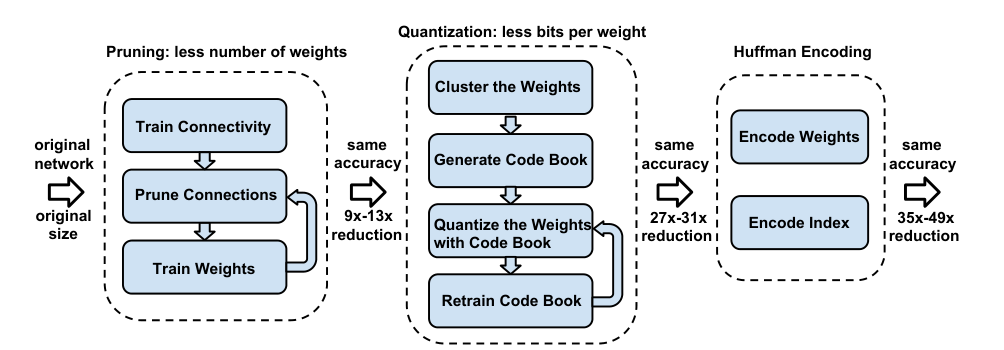
\includegraphics[width=\textwidth]{figures/paper_han_pipeline.png}
\caption{Ba giai đoạn nén trong bài báo gốc: pruning, quantization, rồi Huffman coding \cite{han2016}. Bài này chỉ làm nhánh pruning. Các hệ số \(9\times\)--\(49\times\) là số của bài báo đó, không phải số của Bảng~\ref{tab:results}.}
\label{fig:han-paper}
\end{figure}

\subsection{INT8 PTQ}

INT8 PTQ thay mỗi số thực \(r\) bằng một số nguyên 8 bit \(q\), sau khi mô hình đã huấn luyện xong \cite{jacob2018}.
Không có bước huấn luyện nào nhìn thấy phép làm tròn.
Ánh xạ afin dùng trong bài là
\begin{equation}
S = \frac{r_{\max} - r_{\min}}{255},
\qquad
Z = \mathrm{clip}\!\left(\mathrm{round}\!\left(-128 - \frac{r_{\min}}{S}\right), -128, 127\right),
\label{eq:affine}
\end{equation}
\begin{equation}
q = \mathrm{clip}\!\left(\mathrm{round}(r/S) + Z,\; -128,\; 127\right),
\qquad
\hat r = S(q - Z).
\label{eq:quant}
\end{equation}
\(S\) là thang đo chuyển từ FLOAT32 sang INT8 và \(Z\) là điểm không trên miền INT8. \(S\) và \(Z\) không lưu cho từng trọng số: với activation, mỗi tensor có một cặp \((S, Z)\); với trọng số, mỗi kênh đầu ra có một \(S\) riêng và \(Z = 0\) (per-channel, đối xứng) \cite{jacob2018}.
Vì vậy phần lưu thêm cho \(S\) và \(Z\) rất nhỏ so với số trọng số, và file vẫn giảm khoảng bốn lần.
Miền \(q\) là \([-128, 127]\), tức 256 mã.
Calibration chọn \(r_{\min}\) và \(r_{\max}\) trên một tập ảnh đại diện, rồi bộ chuyển đổi ghi \(S\) và \(Z\) vào file \cite{jacob2018}.

Xét bốn số \(-1.2\), \(-0.4\), \(0.2\) và \(1.0\), không lấy từ mô hình.
Khi đó \(r_{\min} = -1.2\), \(r_{\max} = 1.0\) và \(S = 2.2/255 \approx 0.008627\).
(\ref{eq:affine}) cho \(Z = 11\).
(\ref{eq:quant}) cho \(q\) lần lượt là \(-128\), \(-35\), \(34\) và \(127\).
Bốn giá trị dựng lại là khoảng \(-1.199\), \(-0.397\), \(0.198\) và \(1.001\).
Sai số lớn nhất trong ví dụ này rơi vào \(-0.4\), khoảng \(0.003\).
Ví dụ cho thấy sai số là khoảng cách tới mã gần nhất, và hai đầu miền bị kẹp vào \(-128\) và \(127\).

Mỗi trọng số còn một byte thay vì bốn byte float32, nên kích thước thô và gzip đều có thể giảm.
Phép nhân số nguyên cũng có thể giảm độ trễ trên bộ xử lý trung tâm (central processing unit, CPU) \cite{jacob2018}.
Sai số của cả mạng là sai số làm tròn cộng dồn qua các lớp, sau khi \(S\) và \(Z\) đã khóa.
PTQ không sửa lại trọng số để bù sai số đó.

\begin{figure}[H]
\centering
\begin{tikzpicture}[x=4.5cm,y=1cm,lbl/.style={font=\small}]
  \draw[thick] (-1.45,0) -- (1.25,0);
  \foreach \r/\q/\name in {-1.2/-128/a, -0.4/-35/b, 0.2/34/c, 1.0/127/d}{
    \draw (\r,-0.12) -- (\r,0.12);
    \node[lbl, above] at (\r,0.15) {$\r$};
    \node[lbl, below] at (\r,-0.15) {$\q$};
  }
  \node[lbl] at (-0.1,1.15) {số thực $r$};
  \node[lbl] at (-0.1,-1.15) {mã nguyên $q$};
  \node[lbl, align=center] at (-0.1,-2.05)
    {$S=2.2/255\approx 0.008627$,\quad $Z=11$\\
     256 mã, $q\in[-128,127]$};
\end{tikzpicture}
\caption{Ánh xạ afin INT8 trên bốn số tay. Vị trí trên trục là $r$. Số dưới mỗi vạch là mã $q$. Ví dụ này không lấy từ mô hình.}
\label{fig:int8-mech}
\end{figure}

\noindent\textbf{Áp dụng trong bài.}
Mỗi trọng số float32 chiếm 4 byte và mỗi mã INT8 chiếm 1 byte.
Kích thước thô đi từ 1690.108 KB của mô hình gốc xuống 431.992 KB của dòng INT8.

\noindent\textbf{Mã.}
300 ảnh huấn luyện đầu chọn miền cho (\ref{eq:affine}).
Đầu vào và đầu ra khóa ở int8, đúng miền của (\ref{eq:quant}).

\nopagebreak
{\fontsize{8}{9.2}\selectfont
\begin{verbatim}
def convert_int8(model, name, calibration_count=300):
    def representative():
        for index in range(calibration_count):
            yield [np.ascontiguousarray(x_tr[index:index + 1])]
    converter = tf.lite.TFLiteConverter.from_keras_model(model)
    converter.optimizations = [tf.lite.Optimize.DEFAULT]
    converter.representative_dataset = representative
    converter.target_spec.supported_ops = [tf.lite.OpsSet.TFLITE_BUILTINS_INT8]
    converter.inference_input_type = tf.int8
    converter.inference_output_type = tf.int8
    payload = converter.convert()
    return save_bytes(name, payload), payload
\end{verbatim}}

\begin{figure}[H]
\centering
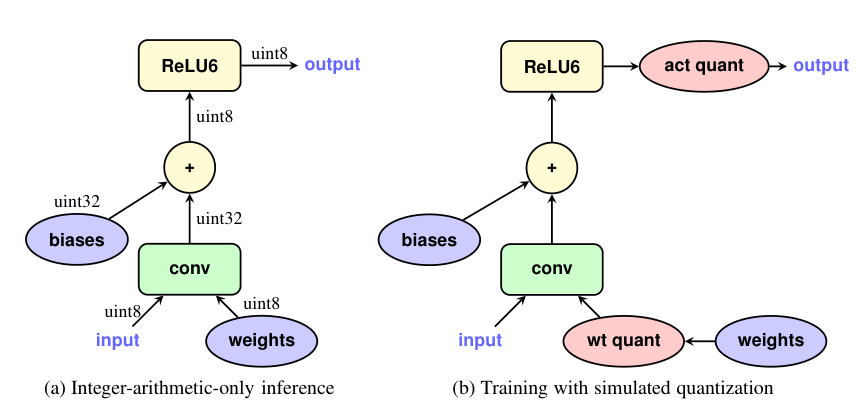
\includegraphics[width=0.92\textwidth]{figures/paper_jacob_conv.png}
\caption{Lớp tích chập ở dạng số nguyên 8 bit khi suy luận, và dạng có nút giả lập lượng tử khi huấn luyện \cite{jacob2018}. Bài này dùng post-training quantization, nên chỉ đi theo panel (a). Panel đo ImageNet của bài báo không được đưa vào.}
\label{fig:jacob-paper}
\end{figure}

\subsection{Knowledge distillation}

Knowledge distillation huấn luyện một mạng nhỏ (học sinh) học theo một mạng lớn đã huấn luyện (thầy) \cite{hinton2015}.
Ý chính: nhãn cứng chỉ nói lớp nào đúng, còn xác suất của thầy nói thêm các lớp sai gần đúng đến mức nào; học sinh học cả hai.
Quy trình gồm năm bước.

\textbf{Bước 1, thầy đưa xác suất.}
Thầy là mô hình gốc float32 (độ chính xác 0.9158), được đóng băng: không cập nhật trọng số.
Với mỗi ảnh huấn luyện, thầy trả về xác suất \(p_i\) cho 10 lớp, tức softmax tại \(T = 1\).

\textbf{Bước 2, làm mềm bằng nhiệt độ \(T\).}
Nếu \(z_i\) là logit lớp \(i\), phân phối mềm là
\begin{equation}
q_i(T) = \frac{\exp(z_i/T)}{\sum_j \exp(z_j/T)}.
\label{eq:temp}
\end{equation}
Vì thầy trả về \(p_i\) thay vì logit, \(q_i(T)\) được tính bằng \(p_i^{1/T}\) rồi chuẩn hóa lại.
\(T\) càng lớn, phân phối càng phẳng, và thông tin về các lớp sai càng rõ.
Ví dụ, với \(T = 4\) và \(p = (0.70,\; 0.20,\; 0.10)\), ba lũy thừa \(1/4\) là khoảng \(0.915\), \(0.669\) và \(0.562\); sau khi chia cho tổng, phân phối mềm là khoảng \(0.426\), \(0.312\) và \(0.262\).
Lớp thắng vẫn là lớp thứ nhất, nhưng hai lớp còn lại không còn bị ép sát không.
Ví dụ này là tính tay trên phương trình~\eqref{eq:temp}, không phải một ảnh của tập đo.

\textbf{Bước 3, học sinh dự đoán.}
Học sinh là \texttt{make\_cnn(8)}: cùng dạng mạng nhưng chỉ 8 kênh, nên ít tham số hơn.
Đầu ra của học sinh cũng được làm mềm với cùng \(T\).

\textbf{Bước 4, hàm mất gộp hai tín hiệu.}
\begin{equation}
L = (1 - \alpha)\,L_{\mathrm{hard}} + \alpha T^{2}\,D_{\mathrm{KL}}.
\label{eq:distill}
\end{equation}
\(L_{\mathrm{hard}}\) là cross-entropy với nhãn cứng: kéo học sinh về đáp án đúng.
\(D_{\mathrm{KL}}\) là độ lệch Kullback--Leibler giữa phân phối mềm của thầy và của học sinh: kéo học sinh về cách thầy phân bố xác suất.
\(\alpha\) chia trọng số giữa hai tín hiệu; bài dùng \(\alpha = 0.5\).
Hệ số \(T^{2}\) giữ biên độ của số hạng mềm khi \(T\) tăng \cite{hinton2015}.

\textbf{Bước 5, chọn epoch và so với đối chứng.}
Epoch được giữ là epoch có độ chính xác kiểm định cao nhất; tập kiểm tra không tham gia lựa chọn này.
Vì học sinh nhỏ hơn thầy, phần lớn mức giảm kích thước đến từ việc ít kênh, không phải từ nhãn mềm.
Do đó cần một học sinh cùng kiến trúc học chỉ trên nhãn cứng (\(\alpha = 0\)); hiệu giữa hai học sinh mới là phần nhãn mềm đóng góp.

Về chi phí: học sinh ít kênh hơn nên kích thước thô, gzip, độ trễ và bộ nhớ đỉnh đều có thể giảm.
Sai số đến từ sức chứa nhỏ hơn của học sinh, không phải từ số không (pruning) hay từ 256 mã (INT8).
\begin{figure}[H]
\centering
\begin{tikzpicture}[
  font=\small,
  box/.style={draw, rounded corners=2pt, align=center, text width=3.35cm,
              minimum height=2.55cm, inner sep=4pt, anchor=center},
  arr/.style={draw, thick, -{Stealth[length=2.2mm]}}
]
  \node[font=\footnotesize, align=center] at (4.7,4.55) {54{,}000 ảnh huấn luyện};
  \node[cylinder, draw, shape border rotate=90, aspect=0.28,
        minimum width=2.5cm, minimum height=1.15cm, align=center,
        font=\small] (data) at (4.7,3.45) {Dữ liệu};
  \node[box] (teacher) at (0,0)
    {\textbf{Mô hình thầy}\\[0.25em]
     CNN float32\\
     độ chính xác\\
     kiểm tra 0.9158};
  \node[box] (mid) at (4.7,0)
    {softmax tại $T=4$\\[0.3em]
     nhãn mềm\\
     gộp với nhãn cứng};
  \node[box] (student) at (9.4,0)
    {\textbf{Học sinh 8 kênh}\\[0.3em]
     $L=(1-\alpha)L_{\mathrm{hard}}$\\
     $\quad+\alpha T^{2}D_{\mathrm{KL}}$\\[0.2em]
     $\alpha=0.5$};
  \draw[arr] (teacher.east) -- (mid.west);
  \draw[arr] (mid.east) -- (student.west);
  \draw[arr] (data.south) ++(-1.15,-0.05) -- (teacher.north);
  \draw[arr] (data.south) ++(1.15,-0.05) -- (student.north);
  \node[font=\footnotesize, align=center] at (0,-2.05)
    {ngoại tuyến\\thầy đóng băng};

  \begin{scope}[shift={(2.6,-4.85)}, x=1cm, y=1cm]
    \node[font=\footnotesize, anchor=south west] at (0,1.85) {ví dụ tay};
    \node[font=\scriptsize, anchor=south west] at (1.7,1.85) {$p=(0.70,\,0.20,\,0.10)$};
    % T=1 group
    \fill[black!18] (0.00,0) rectangle (0.42,1.40);
    \fill[black!18] (0.70,0) rectangle (1.12,0.40);
    \fill[black!18] (1.40,0) rectangle (1.82,0.20);
    \node[font=\scriptsize, above] at (0.21,1.40) {0.70};
    \node[font=\scriptsize, above] at (0.91,0.40) {0.20};
    \node[font=\scriptsize, above] at (1.61,0.20) {0.10};
    \node[font=\scriptsize, below] at (0.21,0) {1};
    \node[font=\scriptsize, below] at (0.91,0) {2};
    \node[font=\scriptsize, below] at (1.61,0) {3};
    \node[font=\scriptsize, anchor=north] at (0.91,-0.42) {$T=1$};
    % T=4 group
    \begin{scope}[shift={(2.7,0)}]
      \fill[black!55] (0.00,0) rectangle (0.42,0.852);
      \fill[black!55] (0.70,0) rectangle (1.12,0.624);
      \fill[black!55] (1.40,0) rectangle (1.82,0.524);
      \node[font=\scriptsize, above] at (0.21,0.852) {0.426};
      \node[font=\scriptsize, above] at (0.91,0.624) {0.312};
      \node[font=\scriptsize, above] at (1.61,0.524) {0.262};
      \node[font=\scriptsize, below] at (0.21,0) {1};
      \node[font=\scriptsize, below] at (0.91,0) {2};
      \node[font=\scriptsize, below] at (1.61,0) {3};
      \node[font=\scriptsize, anchor=north] at (0.91,-0.42) {$T=4$};
    \end{scope}
    \draw[->] (-0.35,0) -- (4.85,0);
    \draw[->] (-0.35,0) -- (-0.35,1.72);
  \end{scope}
\end{tikzpicture}
\caption{Knowledge distillation ngoại tuyến. Mô hình thầy không được cập nhật. Cặp cột là ví dụ tay tại $T=1$ và $T=4$, không phải một ảnh của tập đo.}
\label{fig:kd}
\end{figure}

\noindent\textbf{Áp dụng trong bài.}
Học sinh 8 kênh chưng cất đạt độ chính xác kiểm tra 0.9011.
Học sinh nhãn cứng cùng kiến trúc đạt 0.8974.
Cặp này là một seed; trên năm seed phần tăng là \(-0.0009 \pm 0.0041\) (Mục~\ref{sec:sweep}), nên không có phần tăng đáng tin.
Hai dòng có cùng kích thước thô 415.612 KB.

\noindent\textbf{Mã.}
Hàm mất là (\ref{eq:distill}).
Nhãn mềm là \(p_i^{1/T}\) rồi chuẩn hóa lại, đúng cách đọc (\ref{eq:temp}) khi mô hình gốc đã trả về xác suất.
\texttt{make\_cnn(8)} là kiến trúc chung.
Vòng nhãn cứng dùng cùng kiến trúc, seed 42, 10 epoch, và giữ epoch kiểm định tốt nhất.

\nopagebreak
{\fontsize{8}{9.2}\selectfont
\begin{verbatim}
def make_distill_loss(temperature=4.0, alpha=0.5):
    def loss(y_true, y_pred):
        teacher = tf.clip_by_value(y_true[:, :10], 1e-8, 1.0)
        hard = tf.cast(y_true[:, 10], tf.int32)
        student = tf.clip_by_value(y_pred, 1e-8, 1.0)
        inv_t = 1.0 / temperature
        soft_teacher = tf.pow(teacher, inv_t)
        soft_student = tf.pow(student, inv_t)
        soft_teacher = soft_teacher / tf.reduce_sum(soft_teacher, axis=-1, keepdims=True)
        soft_student = soft_student / tf.reduce_sum(soft_student, axis=-1, keepdims=True)
        kl = tf.reduce_sum(
            soft_teacher * (tf.math.log(soft_teacher) - tf.math.log(soft_student)),
            axis=-1)
        hard_loss = tf_keras.losses.sparse_categorical_crossentropy(hard, y_pred)
        return (1.0 - alpha) * hard_loss + alpha * (temperature ** 2) * kl
    return loss

def make_cnn(width):
    return tf_keras.Sequential([
        tf_keras.layers.Input((28, 28, 1)),
        tf_keras.layers.Conv2D(width, 3, activation="relu", padding="same"),
        tf_keras.layers.MaxPooling2D(),
        tf_keras.layers.Conv2D(2 * width, 3, activation="relu", padding="same"),
        tf_keras.layers.MaxPooling2D(),
        tf_keras.layers.Flatten(),
        tf_keras.layers.Dense(128, activation="relu"),
        tf_keras.layers.Dropout(0.3),
        tf_keras.layers.Dense(10, activation="softmax"),
    ])

tf.random.set_seed(42)
np.random.seed(42)
student = make_cnn(8)
student.compile(
    optimizer="adam",
    loss="sparse_categorical_crossentropy",
    metrics=["accuracy"],
)
best = {"acc": -1.0, "epoch": None, "weights": None}
for epoch in range(10):
    student.fit(x_tr, y_tr, epochs=1, batch_size=128, shuffle=True, verbose=2)
    acc = float((student.predict(x_val, batch_size=256, verbose=0).argmax(1) == y_val).mean())
    if acc > best["acc"]:
        best = {"acc": acc, "epoch": epoch + 1,
                "weights": [item.copy() for item in student.get_weights()]}
student.set_weights(best["weights"])
\end{verbatim}}

\begin{figure}[H]
\centering
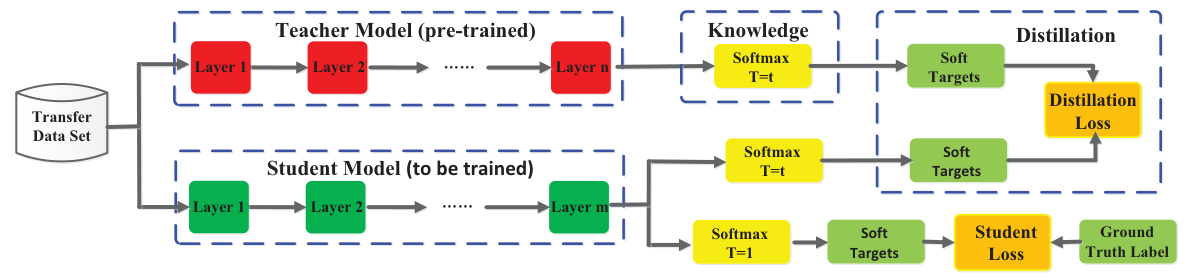
\includegraphics[width=\textwidth]{figures/paper_gou_hinton.png}
\caption{Kiến trúc chưng cất chuẩn của Hinton et al., vẽ lại trong bài tổng quan \cite{gou2021,hinton2015}. Thầy đã huấn luyện đưa nhãn mềm; học sinh học nhãn mềm cùng nhãn cứng. Hình này không phải mạng Fashion-MNIST của bài.}
\label{fig:gou-paper}
\end{figure}

\section{Phương pháp}

Pipeline xuất phát từ một mô hình gốc float32 và tách thành các nhánh độc lập.
Pruning và distillation nhận một mạng và trả về một mạng.
INT8 PTQ nhận một mạng và trả về file TFLite, nên INT8 PTQ đứng cuối nếu nó có trong thứ tự.
Học sinh nhãn cứng không đi qua mô hình gốc ở bước huấn luyện.
Nó chỉ dùng cùng kiến trúc với học sinh chưng cất, để so kích thước và độ chính xác.
Mọi nhánh kết thúc bằng một file TFLite rồi đi vào cùng một phép đo.

\begin{figure}[H]
\centering
\begin{tikzpicture}[
  font=\footnotesize,
  file/.style={draw, rounded corners=2pt, align=center,
               text width=3.35cm, minimum height=1.12cm,
               inner sep=3pt, fill=black!6},
  last/.style={file, fill=black!15},
  ctrl/.style={draw, dashed, rounded corners=2pt, align=center,
               text width=13.15cm, minimum height=0.95cm, inner sep=3pt},
  arr/.style={draw, thick, -{Stealth[length=2.1mm]}},
  tag/.style={font=\scriptsize, align=center, inner sep=1.4pt, fill=white}
]
  \node[file, text width=4.2cm] (base) at (0,0) {float baseline};

  \node[file] (pr) at (-4.9,-2.55) {pruned};
  \node[file] (st) at (4.9,-2.55) {distilled student};

  \node[last] (pi) at (-4.9,-5.15) {pruned INT8};
  \node[last] (i8) at (0,-5.15) {INT8};
  \node[last] (sk) at (4.9,-5.15) {distilled pruned INT8\\stacked, default config};

  \draw[arr] (base.south) -- (pr.north);
  \draw[arr] (base.south) -- (i8.north);
  \draw[arr] (base.south) -- (st.north);
  \node[tag, anchor=south east] at (-2.35,-0.95) {pruning};
  \node[tag, anchor=west] at (0.22,-1.25) {INT8};
  \node[tag, anchor=south west] at (2.35,-0.95) {distillation};

  \draw[arr] (pr.south) -- (pi.north);
  \node[tag] at (-4.9,-3.85) {INT8};
  \draw[arr] (st.south) -- (sk.north);
  \node[tag] at (4.9,-3.85) {pruning rồi INT8};

  \node[draw, rounded corners=2pt, fill=black!4, align=center,
        text width=13.15cm, minimum height=0.95cm] (meas) at (0,-6.75)
    {cùng một phép đo: độ chính xác, kích thước tệp .tflite, gzip, p50, p95, bộ nhớ đỉnh};
  \draw[arr] (pi.south) -- (pi.south |- meas.north);
  \draw[arr] (i8.south) -- (i8.south |- meas.north);
  \draw[arr] (sk.south) -- (sk.south |- meas.north);

  \node[ctrl] at (0,-8.15)
    {small from-scratch: cùng kiến trúc với distilled student, không đi qua float baseline, cùng phép đo};
\end{tikzpicture}
\caption{Pipeline từ float baseline qua pruning, INT8 và distillation; pruning rồi INT8 thành pruned INT8, distillation rồi pruning rồi INT8 thành distilled pruned INT8 và stacked, default config. Hộp đứt nét là small from-scratch, cùng kiến trúc, không đi qua float baseline.}
\label{fig:pipeline}
\end{figure}

Ảnh được chia một lần, không xáo trước khi cắt.
Tập huấn luyện là 54{,}000 ảnh đầu của tập huấn luyện chính thức.
Tập kiểm định là 6{,}000 ảnh cuối của tập đó.
Tập kiểm tra là 10{,}000 ảnh kiểm tra chính thức.
Mỗi ảnh được chia cho 255 và thêm một trục kênh.

\filbreak
\noindent\textbf{Mã.}
Không xáo trước khi cắt.

\nopagebreak
{\fontsize{8}{9.2}\selectfont
\begin{verbatim}
tf.random.set_seed(42)
np.random.seed(42)
(x_train_full, y_train_full), (x_te, y_te) = (
    tf.keras.datasets.fashion_mnist.load_data())
x_train_full = (x_train_full / 255.0).astype("float32")[..., None]
x_te = (x_te / 255.0).astype("float32")[..., None]
x_tr, y_tr = x_train_full[:-6000], y_train_full[:-6000]
x_val, y_val = x_train_full[-6000:], y_train_full[-6000:]
assert len(x_tr) == 54000 and len(x_val) == 6000 and len(x_te) == 10000
\end{verbatim}}

Mô hình học sinh 8 kênh có tích chập 8 kênh, gộp cực đại, tích chập 16 kênh, gộp cực đại, trải phẳng, tầng dày 128 đơn vị với rectified linear unit (ReLU), Dropout 0.3, và tầng dày 10 đơn vị với softmax.
Kernel tích chập có cạnh 3 và đệm same.
Mô hình gốc không được dựng lại trong lần đo này.
Mọi dòng nén hoặc nạp lại mô hình gốc, hoặc nạp đúng mạng mà nhánh trước của cùng một thứ tự vừa trả về.

Bảng~\ref{tab:hyper} gom siêu tham số.
Pruning trên mô hình gốc dùng nhãn cứng, tần suất 100, và giữ epoch cuối.
Pruning trên học sinh đã chưng cất dùng mất mát (\ref{eq:distill}), tần suất 1, và cũng giữ epoch cuối.
Lần cấu hình mặc định cắt học sinh đã lưu tới \(s_f = 0.70\).
Lần đã chỉnh huấn luyện học sinh mới trong cùng lượt và cắt tới \(s_f = 0.30\).
Lịch trên mô hình gốc vẫn có \(s_f = 0.70\).
Cả hai lịch có \(s_i = 0\), \(p = 3\), và kết thúc đúng bước cuối của 4 epoch với cỡ lô 128, như (\ref{eq:poly}).
INT8 PTQ dùng 300 ảnh huấn luyện đầu để calibration, toán tử nguyên 8 bit, và khóa cả đầu vào lẫn đầu ra ở int8.
Hai học sinh dùng cùng số epoch, cùng cỡ lô, và tốc độ học mặc định của Adam trong thư viện.
Với \(\alpha = 0.5\), một nửa (\ref{eq:distill}) vẫn là nhãn cứng.

\begin{table}[H]
\centering
\caption{Siêu tham số đã chốt của pruning, INT8, distillation, small from-scratch, pruned INT8, distilled pruned INT8 và stacked, default config. Adam của hai học sinh là mặc định của thư viện, không ghi một tốc độ học riêng.}
\label{tab:hyper}
\begin{tabularx}{\textwidth}{|l|Y|}
\hline
Nhánh & Configuration \\ \hline
Chia dữ liệu & 54{,}000 huấn luyện, 6{,}000 kiểm định, 10{,}000 kiểm tra; seed 42 trước khi dựng học sinh \\ \hline
Pruning, mô hình gốc & \(s_f = 0.70\), PolynomialDecay, \(p = 3\), tần suất 100, 4 epoch, lô 128, Adam \(1\times 10^{-4}\), nhãn cứng, giữ epoch cuối \\ \hline
Pruning, học sinh, cấu hình mặc định & nạp học sinh distillation đã lưu; \(s_f = 0.70\), PolynomialDecay, \(p = 3\), tần suất 1, 4 epoch, lô 128, Adam \(1\times 10^{-4}\), mất mát (\ref{eq:distill}), giữ epoch cuối \\ \hline
Pruning, học sinh, cấu hình đã chỉnh & học sinh \texttt{make\_cnn(8)} mới trong cùng lượt, 10 epoch, giữ epoch validation tốt nhất; \(s_f = 0.30\), PolynomialDecay, \(p = 3\), tần suất 1, 4 epoch, lô 128, Adam \(1\times 10^{-4}\), mất mát (\ref{eq:distill}), giữ epoch cuối \\ \hline
INT8 PTQ & 300 ảnh huấn luyện đầu, full INT8, đầu vào và đầu ra int8 \\ \hline
Distillation & \(T = 4\), \(\alpha = 0.5\), học sinh 8 kênh, 10 epoch, lô 128, Adam mặc định, giữ epoch kiểm định tốt nhất \\ \hline
Học sinh nhãn cứng & cùng kiến trúc và cùng 10 epoch, nhãn cứng, Adam mặc định, giữ epoch kiểm định tốt nhất \\ \hline
\end{tabularx}
\end{table}

\section{Thực nghiệm}

Độ chính xác kiểm tra là tỉ lệ đúng trên 10{,}000 ảnh kiểm tra.
Độ giảm, tính bằng pp, là \((0.9158 - a)\times 100\), với \(a\) là độ chính xác kiểm tra của dòng đó.
Mốc 0.9158 là độ chính xác của mô hình gốc float32.
Kích thước thô là số byte của file TFLite.
KB lấy số byte chia cho 1000.
MB lấy số byte chia cho \(1{,}000{,}000\).
Gzip là kích thước sau khi nén mức 9 với mốc thời gian bằng 0.
Phần cắt gzip là phần trăm gzip đã bỏ đi so với gzip của mô hình gốc.
Phần cắt thô là phần trăm kích thước thô đã bỏ đi so với 1690.108 KB của cùng dòng float baseline.
Dòng mô hình gốc được gán cả hai phần cắt bằng 0, vì nó là mẫu số.

\noindent\textbf{Mã.}
KB là byte chia 1000.
MB trong bảng in là KB chia 1000.
Mã dưới đây là phép đo đã chạy: \texttt{size\_cut} là phần cắt gzip, và \texttt{bar\_flags} chỉ so độ giảm với 2 pp và phần cắt gzip với 50 phần trăm.
Phần cắt thô và vạch Keras–TFLite được chấm trong báo cáo từ số đã lưu, như mục Điều kiện đạt phía dưới.

\nopagebreak
{\fontsize{8}{9.2}\selectfont
\begin{verbatim}
def gzip_size(payload):
    return len(gzip.compress(payload, compresslevel=9, mtime=0))

raw = len(payload)
gzip_n = gzip_size(payload)
row["raw_kb"] = raw / 1000
row["gzip_kb"] = gzip_n / 1000
row["size_cut"] = (BASE_GZIP - gzip_n) / BASE_GZIP * 100

def bar_flags(row):
    return row["loss_pp"] <= 2.0, row["size_cut"] >= 50.0

f"{row['raw_kb']:10.3f} {row['raw_kb']/1000:10.6f} "
f"{row['gzip_kb']:10.3f} {row['gzip_kb']/1000:10.6f} "
\end{verbatim}}

Cột \texttt{verdict} của \texttt{results/results.csv} vẫn ghi PASS cho dòng pruned, vì \texttt{bar\_flags} chỉ kiểm độ giảm và phần cắt gzip.
Bảng~\ref{tab:results} áp vạch thô tính từ \texttt{raw\_KB} đã lưu, nên cùng dòng đó ghi FAIL (raw).

Độ trễ là thời gian một lần suy luận (một ảnh, batch = 1), tính bằng mili giây.
Mỗi tiến trình chạy 20 lần khởi động (warm-up) và bỏ đi, sau đó đo 200 lần lặp.
Bộ khởi động là nhóm riêng chạy trước, không nằm trong 200 lần đo.
200 thời gian đo được sắp xếp từ nhanh đến chậm.
p50 (phân vị 50, trung vị) là giá trị ở giữa danh sách: một nửa số lần chạy nhanh hơn nó,
nên p50 cho biết một lần chạy điển hình.
p95 (phân vị 95) là giá trị mà 95\% số lần chạy không vượt quá,
nên p95 cho biết đuôi chậm, tức 5\% lần chạy chậm nhất.
Bài không dùng trung bình vì vài lần chạy chậm bất thường (hệ điều hành ngắt, cache miss)
sẽ kéo trung bình lên; trung vị không bị ảnh hưởng bởi các lần đó,
còn p95 cố ý giữ chúng lại để thấy.
Phép đo lặp ba lần, và bảng báo cáo trung vị của ba giá trị p50 và ba giá trị p95.


\texttt{VmHWM} (high-water mark) là mức đỉnh của bộ nhớ thường trú
(resident set size, RSS) mà Linux ghi cho mỗi tiến trình,
tức lượng RAM thật lớn nhất tiến trình đã chiếm.
Đây không phải bộ nhớ ảo; đỉnh bộ nhớ ảo là \texttt{VmPeak}, một đại lượng khác.
Một tiến trình Python đã chiếm RAM trước khi nạp mô hình
(trình thông dịch, NumPy, thư viện TFLite).
Để chỉ giữ phần do mô hình gây ra, bài chạy ba tiến trình rỗng (không nạp mô hình)
và ba tiến trình có mô hình, lấy trung vị \texttt{VmHWM} của mỗi nhóm, rồi lấy hiệu:
\[
  \text{bộ nhớ đỉnh} = \operatorname{median}(\texttt{VmHWM}_{\text{có mô hình}})
                     - \operatorname{median}(\texttt{VmHWM}_{\text{rỗng}}).
\]

\paragraph{Điều kiện đạt.}
Ba vạch bắt buộc.
Vạch độ chính xác và vạch kích thước chấm từng dòng nén.
Vạch thứ ba chấm một lần trên mô hình float, không chấm theo từng dòng.
\begin{enumerate}
  \item độ giảm độ chính xác không quá 2 pp so với mô hình gốc,
        tức \(0.9158 - a \le 0.02\), hay \(a \ge 0.8958\);
  \item phần cắt kích thước không dưới 50\%, kiểm trên cả hai đại lượng:
        phần cắt thô \(1 - \text{raw}_{\text{dòng}} / \text{raw}_{\text{gốc}} \ge 0.5\),
        với \(\text{raw}_{\text{gốc}} = 1690.108\) KB,
        và phần cắt gzip \(1 - \text{gzip}_{\text{dòng}} / \text{gzip}_{\text{gốc}} \ge 0.5\),
        với \(\text{gzip}_{\text{gốc}} = 1567.603\) KB;
  \item Tương đương sau chuyển đổi: sai lệch đầu ra lớn nhất Keras vs TFLite (float, trước lượng tử hoá) \(\le 1\times 10^{-4}\).
\end{enumerate}
Vạch độ chính xác và vạch kích thước không áp vào float baseline vì đó là mốc để đo:
độ giảm của nó là 0.00 pp, phần cắt thô là 0.00\% và phần cắt gzip là 0.00\%.
Hàm \texttt{bar\_flags} trong mã phía trên chỉ trả về cờ độ giảm và cờ phần cắt gzip đã tính lúc đo.
Phần cắt thô trong Bảng~\ref{tab:results} được tính từ cột \texttt{raw\_KB} đã lưu.

\begin{table}[H]
\centering
\caption{Giao thức đo dùng chung cho float baseline, small from-scratch, pruned, INT8, distilled student, pruned INT8, distilled pruned INT8 và stacked, default config. Độ trễ trung vị (p50) và độ trễ phân vị 95 (p95) đo trên CPU, batch = 1, một luồng, là trung vị của ba lần đo.}
\label{tab:protocol}
\begin{tabularx}{\textwidth}{|l|Y|}
\hline
Hạng mục & Giá trị \\ \hline
Thiết bị & CPU 13th Gen Intel(R) Core(TM) i9-13900HX \\ \hline
Luồng của thông dịch & 1 \\ \hline
Độ chính xác & 10{,}000 ảnh kiểm tra; lô 256 nếu file nhận, không thì lô 1 \\ \hline
Độ trễ & ảnh kiểm tra đầu tiên; lô 1; vùng bấm giờ là nạp tensor, gọi suy luận, rồi đọc tensor \\ \hline
Khởi động & 20 lần, không ghi vào phân vị \\ \hline
Lần bấm giờ & 200 lần trong mỗi lượt \\ \hline
Số lượt & 3; p50 và p95 ghi vào bảng là trung vị của ba lượt \\ \hline
Gzip & mức 9, mốc thời gian 0 \\ \hline
Bộ nhớ đỉnh & trung vị \texttt{VmHWM} của 3 tiến trình mô hình trừ trung vị của 3 tiến trình rỗng; sàn 34944 kB \\ \hline
Ngưỡng đạt & độ giảm \(\le 2\) pp; phần cắt thô \(\ge 50\) phần trăm; phần cắt gzip \(\ge 50\) phần trăm. Vạch Keras vs TFLite (float, trước lượng tử hoá) \(\le 1\times 10^{-4}\), kiểm một lần trên mô hình float, không theo từng dòng \\ \hline
\end{tabularx}
\end{table}

\filbreak
\noindent\textbf{Mã.}
20 lần đầu gọi cùng ba bước và không ghi thời gian.
200 lần sau mới vào danh sách mẫu.
Mỗi lần là một ảnh.
Ba lượt; giá trị ghi vào bảng là giá trị giữa.

\nopagebreak
{\fontsize{8}{9.2}\selectfont
\begin{verbatim}
def latency_medians(path):
    interpreter = make_interpreter(path)
    detail = interpreter.get_input_details()[0]
    if list(detail["shape"]) != [1, 28, 28, 1]:
        interpreter.resize_tensor_input(detail["index"], [1, 28, 28, 1], strict=True)
        interpreter.allocate_tensors()
    sample = x_te[0][None, ...]
    p50, p95 = [], []
    for _ in range(3):
        input_detail = interpreter.get_input_details()[0]
        output_detail = interpreter.get_output_details()[0]
        feed = quantize_input(sample, input_detail)
        for _ in range(20):
            interpreter.set_tensor(input_detail["index"], feed)
            interpreter.invoke()
            interpreter.get_tensor(output_detail["index"])
        samples = []
        for _ in range(200):
            start = time.perf_counter()
            interpreter.set_tensor(input_detail["index"], feed)
            interpreter.invoke()
            interpreter.get_tensor(output_detail["index"])
            samples.append((time.perf_counter() - start) * 1000)
        p50.append(float(np.percentile(samples, 50)))
        p95.append(float(np.percentile(samples, 95)))
    p50.sort(); p95.sort()
    return p50[1], p95[1]
\end{verbatim}}

Tiến trình đo bộ nhớ chỉ nạp bộ bao thông dịch và NumPy, không nạp cả thư viện huấn luyện.
Tiến trình rỗng không nhận file mô hình.
Ba tiến trình rỗng cho \texttt{VmHWM} 34932 kB, 34944 kB và 35108 kB, nên sàn là trung vị 34944 kB.
Cột bộ nhớ trong bảng kết quả là hiệu đã tính, không phải \texttt{VmHWM} thô.

\noindent\textbf{Mã.}
Ba tiến trình rỗng cho sàn.
Ba tiến trình có mô hình cho mức cao.
Tiến trình con gọi suy luận 200 lần rồi đọc \texttt{VmHWM}.

\nopagebreak
{\fontsize{8}{9.2}\selectfont
\begin{verbatim}
def peak_delta(model_path):
    global FLOOR_KB
    if FLOOR_KB is None:
        empty = sorted(_vmhwm_once("") for _ in range(3))
        FLOOR_KB = empty[1]
    readings = sorted(_vmhwm_once(model_path) for _ in range(3))
    return readings[1], readings[1] - FLOOR_KB

for _ in range(200):
    interp.SetTensor(in_idx, feed)
    interp.Invoke()
    interp.GetTensor(out_idx, 0)
\end{verbatim}}

Vạch thứ ba, tương đương sau chuyển đổi, đạt.
Sai lệch đầu ra lớn nhất Keras vs TFLite (float, trước lượng tử hoá), trên cả 10{,}000 ảnh kiểm tra, là \(1.7583370208740234\times 10^{-6}\), dưới ngưỡng \(1\times 10^{-4}\).
Số này là trường \texttt{value} của \texttt{results/equivalence.json}.
Vạch này kiểm một lần trên mô hình float, không kiểm theo từng dòng của Bảng~\ref{tab:results}.

\section{Kết quả và bàn luận}

Mọi số trong mục này lấy từ bảng kết quả.
Sáu dòng đầu là phần so sánh cuối của sổ đo.
Dòng distilled pruned INT8 là lần xếp đã chỉnh: distillation, pruning với độ thưa cuối 0.30, rồi INT8.
Dòng stacked, default config là lần xếp cùng thứ tự với độ thưa cuối 0.70.
Phụ lục A ghi file của từng dòng.
p50 và p95 dưới đây là hai cột của bảng này.

Bảng~\ref{tab:results} chấm từng dòng nén trên ba điều kiện: độ giảm, phần cắt thô và phần cắt gzip.
Small from-scratch, INT8, distilled student, pruned INT8 và distilled pruned INT8 có kết quả PASS.
Dòng pruned qua vạch độ chính xác và vạch gzip, và FAIL ở vạch thô.
Dòng stacked, default config qua vạch thô và vạch gzip, và FAIL ở vạch độ chính xác.
Dòng float baseline là mốc, với độ chính xác 0.9158, độ giảm 0.00 pp, kích thước thô 1690.108 KB, gzip 1567.603 KB, p50 bằng 0.155 ms, p95 bằng 0.226 ms, và bộ nhớ đỉnh 7108 kB.
Vạch Keras–TFLite không có cột trong bảng này.

\begin{table}[H]
\centering
\caption{Độ chính xác trên tập kiểm tra, độ giảm so với 0.9158 (pp), kích thước tệp .tflite (KB và MB), kích thước tệp .tflite sau nén gzip (KB và MB), phần trăm kích thước thô đã cắt, phần trăm gzip đã cắt, độ trễ trung vị (p50, ms), độ trễ phân vị 95 (p95, ms) và bộ nhớ đỉnh (VmHWM trừ tiến trình rỗng, kB) của float baseline, small from-scratch, pruned, INT8, distilled student, pruned INT8, distilled pruned INT8 và stacked, default config. Cột Kết quả là PASS khi độ giảm không quá 2 pp, phần cắt thô không dưới 50 phần trăm và phần cắt gzip không dưới 50 phần trăm; FAIL (raw) trượt vạch thô và FAIL (acc) trượt vạch độ chính xác. Độ trễ đo trên CPU, batch = 1, một luồng, trung vị của ba lần đo.}
\label{tab:results}
\resizebox{\textwidth}{!}{%
\begin{tabular}{|l|r|r|r|r|r|r|r|r|r|r|r|l|}
\hline
Dòng & Test & Loss & Raw KB & Raw MB & Gzip KB & Gzip MB & Raw cut & Gzip cut & p50 & p95 & Vm & Kết quả \\ \hline
float baseline & 0.9158 & 0.00 & 1690.108 & 1.690108 & 1567.603 & 1.567603 & 0.00 & 0.00 & 0.155 & 0.226 & 7108 & reference \\ \hline
small from-scratch & 0.8974 & 1.84 & 415.612 & 0.415612 & 384.088 & 0.384088 & 75.41 & 75.50 & 0.025 & 0.028 & 4692 & PASS \\ \hline
pruned & 0.9099 & 0.59 & 1690.108 & 1.690108 & 622.146 & 0.622146 & 0.00 & 60.31 & 0.179 & 0.261 & 7244 & FAIL (raw) \\ \hline
INT8 & 0.9150 & 0.08 & 431.992 & 0.431992 & 383.123 & 0.383123 & 74.44 & 75.56 & 0.068 & 0.079 & 4684 & PASS \\ \hline
distilled student & 0.9011 & 1.47 & 415.612 & 0.415612 & 384.058 & 0.384058 & 75.41 & 75.50 & 0.025 & 0.029 & 4636 & PASS \\ \hline
pruned INT8 & 0.9102 & 0.56 & 431.992 & 0.431992 & 181.994 & 0.181994 & 74.44 & 88.39 & 0.070 & 0.094 & 4648 & PASS \\ \hline
distilled pruned INT8 & 0.8992 & 1.66 & 111.424 & 0.111424 & 87.025 & 0.087025 & 93.41 & 94.45 & 0.008 & 0.009 & 4012 & PASS \\ \hline
stacked, default config & 0.8855 & 3.03 & 111.424 & 0.111424 & 49.483 & 0.049483 & 93.41 & 96.84 & 0.015 & 0.028 & 4016 & FAIL (acc) \\ \hline
\end{tabular}}
\end{table}

Ba phép đứng riêng cho ba kiểu giảm khác nhau.
INT8 của mô hình gốc đi từ độ chính xác 0.9158 xuống 0.9150, tức giảm 0.08 pp.
Kích thước thô đi từ 1690.108 KB xuống 431.992 KB.
Gzip đi từ 1567.603 KB xuống 383.123 KB, tức cắt 75.56 phần trăm.
p50 đi từ 0.155 ms xuống 0.068 ms, và p95 đi từ 0.226 ms xuống 0.079 ms.
Bộ nhớ đỉnh đi từ 7108 kB xuống 4684 kB.
Đây là phép đơn giữ độ chính xác sát mốc nhất, và qua vạch thô lẫn vạch gzip: phần cắt thô 74.44 phần trăm, phần cắt gzip 75.56 phần trăm.

Pruning trên mô hình gốc không đổi kích thước thô: cả hai dòng float đều là 1690.108 KB và 1.690108 MB.
Gzip giảm từ 1567.603 KB xuống 622.146 KB, tức cắt 60.31 phần trăm, nên dòng này qua vạch gzip.
Phần cắt thô là 0.00 phần trăm, nên dòng này FAIL ở vạch thô.
Độ chính xác là 0.9099, giảm 0.59 pp.
p50 lại tăng từ 0.155 ms lên 0.179 ms, và p95 tăng từ 0.226 ms lên 0.261 ms.
Bộ nhớ đỉnh tăng từ 7108 kB lên 7244 kB.
Vì vậy pruning ở dạng mảng float đủ phần tử cắt được gzip, nhưng không cắt file thô và không làm lần suy luận giữa nhanh hơn.
Hình~\ref{fig:hist} chỉ minh họa việc đưa trọng số nhỏ về không trên một bản sao.
Hình đó không phải dòng pruned của Bảng~\ref{tab:results}.

Hai học sinh 8 kênh có cùng kích thước thô 415.612 KB, tức 0.415612 MB.
Học sinh nhãn cứng đạt độ chính xác 0.8974, giảm 1.84 pp, gzip 384.088 KB, cắt 75.50 phần trăm.
Học sinh chưng cất đạt 0.9011, giảm 1.47 pp, gzip 384.058 KB, cũng cắt 75.50 phần trăm.
Hiệu hai độ giảm là \(1.84 - 1.47 = 0.37\) pp, lấy cùng mốc 0.9158.
p50 của cả hai là 0.025 ms.
p95 là 0.028 ms và 0.029 ms.
Bộ nhớ đỉnh là 4692 kB và 4636 kB.
Cùng kiến trúc, cặp file trong bảng lệch 0.37 pp.
Cặp 0.9011 và 0.8974 là một seed; trên năm seed phần tăng là \(-0.0009 \pm 0.0041\) (Mục~\ref{sec:sweep}), nên không có phần tăng đáng tin.
Cả hai vẫn PASS, vì 1.84 pp còn dưới vạch 2 pp, phần cắt thô là 75.41 phần trăm và phần cắt gzip là 75.50 phần trăm.
Phần lớn chỗ giảm kích thước đến từ số kênh, không đến từ nhãn mềm.

Xếp pruning rồi INT8 trên mô hình gốc không cộng hai độ giảm.
INT8 một mình giảm 0.08 pp.
Pruning một mình giảm 0.59 pp.
Dòng xếp này giảm 0.56 pp, sát độ giảm của pruning và thấp hơn tổng \(0.59 + 0.08 = 0.67\) pp.
Kích thước thô là 431.992 KB, bằng đúng INT8 một mình.
Gzip còn 181.994 KB, cắt 88.39 phần trăm, thấp hơn 383.123 KB của INT8 một mình.
Phần cắt thô là 74.44 phần trăm, bằng INT8 một mình, nên dòng này qua vạch thô và vạch gzip.
p50 là 0.070 ms, sát 0.068 ms của INT8 một mình, và p95 là 0.094 ms.
Bộ nhớ đỉnh là 4648 kB, sát 4684 kB.
Trên mô hình rộng, INT8 quyết định kích thước thô, độ trễ và bộ nhớ.
Pruning quyết định phần gzip bị cắt thêm, và gần như quyết định luôn độ giảm độ chính xác.

Xếp distillation, pruning và INT8 trên học sinh dùng độ thưa cuối 0.30, thấp hơn 0.70 của mô hình gốc.
Học sinh chưng cất đã giảm 1.47 pp trước khi bị pruning.
Dòng xếp đủ ba bước còn độ chính xác 0.8992, tức giảm 1.66 pp.
Phần tăng thêm so với chính học sinh đó là \(1.66 - 1.47 = 0.19\) pp.
Mức 0.19 pp nhỏ hơn độ giảm 0.59 pp của pruning trên mô hình gốc.
Thô còn 111.424 KB, tức 0.111424 MB, vì INT8 vẫn ghi đủ mã 8 bit cho từng trọng số.
Gzip còn 87.025 KB, cắt 94.45 phần trăm so với 1567.603 KB.
Phần cắt thô là 93.41 phần trăm.
p50 còn 0.008 ms, p95 còn 0.009 ms, và bộ nhớ đỉnh còn 4012 kB.
Trong các dòng PASS cả ba vạch trên dòng, đây là gzip nhỏ nhất và p50 thấp nhất.

Hai lần xếp dùng cùng lịch PolynomialDecay với \(s_i = 0\), \(p = 3\), tần suất 1, 4 epoch pruning, mất mát distillation \(T = 4\), \(\alpha = 0.5\), Adam \(1\times 10^{-4}\), và 300 ảnh hiệu chuẩn.
Điểm khác là điểm xuất phát của học sinh và độ thưa cuối.
Lần cấu hình mặc định nạp học sinh distillation đã lưu, rồi cắt tới \(s_f = 0.70\): accuracy 0.8855, giảm 3.03 pp, phần cắt thô 93.41 phần trăm, gzip 49.483 KB, cắt 96.84 phần trăm, p50 0.015 ms, bộ nhớ đỉnh 4016 kB, kết quả FAIL (acc).
Lần đã chỉnh huấn luyện học sinh \texttt{make\_cnn(8)} mới trong cùng lượt, giữ epoch validation tốt nhất, rồi cắt tới \(s_f = 0.30\): accuracy 0.8992, giảm 1.66 pp, phần cắt thô 93.41 phần trăm, gzip 87.025 KB, cắt 94.45 phần trăm, p50 0.008 ms, bộ nhớ đỉnh 4012 kB, kết quả PASS.
Gzip của cấu hình mặc định là 49.483 KB, còn gzip của lần đã chỉnh là 87.025 KB.
Độ giảm 3.03 pp nằm trên vạch 2 pp.
Hai thiết lập khác nhau ở hai núm cùng lúc (điểm xuất phát học sinh và \(s_f\)), nên bảng không tách được đóng góp của từng núm.
Theo phép quét \(s_f\) ở Mục~\ref{sec:sweep}, giảm \(s_f\) là nguyên nhân chính có khả năng nhất; học sinh huấn luyện lại chỉ thay đổi trong biên độ nhiễu seed (khoảng \(\pm 0.002\)).
\(s_f = 0.30\) nằm ngoài khoảng quét 0.5--0.9.

Hình~\ref{fig:scatter} đặt gzip trên trục ngang và độ giảm trên trục dọc.
Vạch ngang là 2 pp.
Vạch dọc là một nửa gzip của mô hình gốc, tức vạch cắt gzip 50 phần trăm.
Hình này không vẽ phần cắt thô.
Small from-scratch, INT8, distilled student, pruned INT8 và distilled pruned INT8 nằm dưới vạch ngang và bên trái vạch dọc, và cũng qua vạch thô.
Điểm pruned cũng nằm trong vùng đó trên hình này, vì gzip cắt 60.31 phần trăm và độ giảm là 0.59 pp, nhưng phần cắt thô là 0.00 phần trăm nên dòng FAIL (raw).
Điểm stacked, default config có độ giảm 3.03 pp, nên nằm trên vạch ngang, với gzip 49.483 KB, dù phần cắt thô 93.41 phần trăm và phần cắt gzip 96.84 phần trăm đều qua vạch kích thước.
Hình~\ref{fig:p50} xếp p50 của tám dòng.
p50 của cấu hình mặc định là 0.015 ms.
Cột của dòng xếp ba bước là cột thấp nhất, 0.008 ms.
Cột của pruning trên mô hình gốc cao hơn cột của mô hình gốc, đúng với 0.179 ms so với 0.155 ms.
Đổi lấy kích thước vì vậy không phải lúc nào cũng đổi lấy tốc độ.
Dòng cân bằng nhất trong bảng là pruned INT8: giảm 0.56 pp, vẫn dưới 2 pp, và cắt 88.39 phần trăm gzip, trong khi p50 là 0.070 ms.

\figframe{Kích thước tệp .tflite sau nén gzip (KB) và độ giảm độ chính xác trên tập kiểm tra (pp) của float baseline, small from-scratch, pruned, INT8, distilled student, pruned INT8, distilled pruned INT8 và stacked, default config. Vạch ngang đứt là 2 pp và vạch dọc đứt là gzip sau khi cắt 50 phần trăm. Phần cắt thô không có trên hình này; cột Raw cut của Bảng~\ref{tab:results} mới là vạch thô.\label{fig:scatter}}{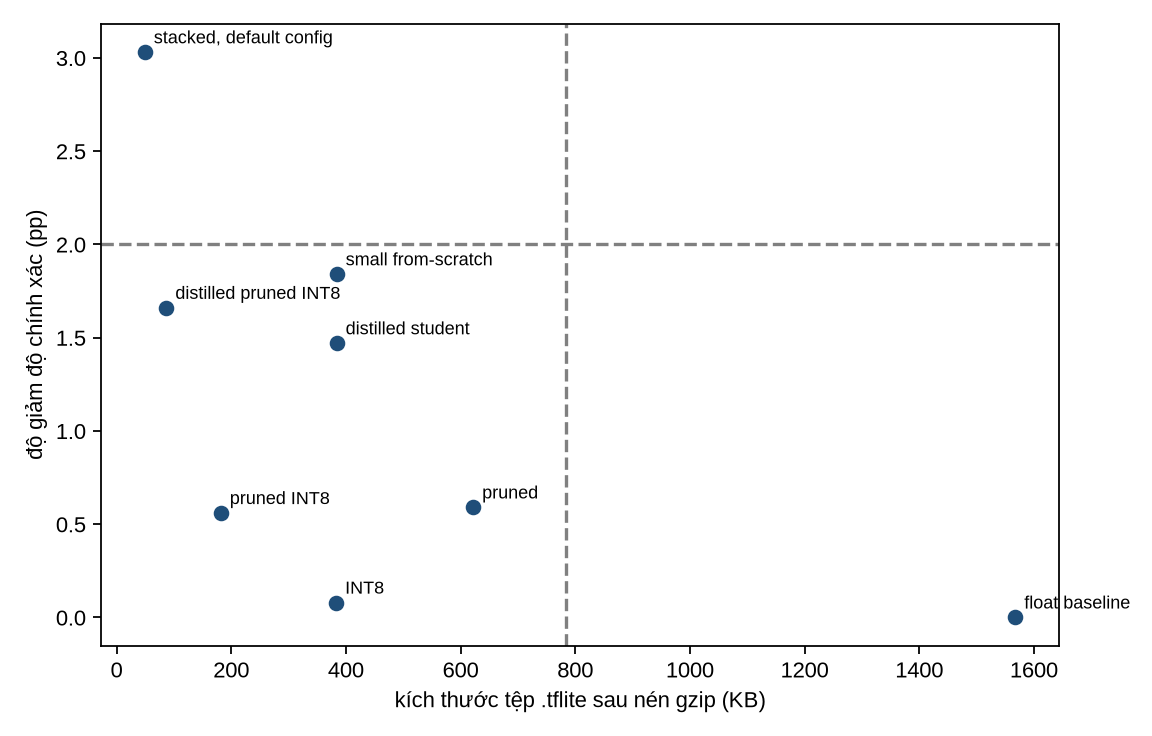
\includegraphics[width=0.88\textwidth]{figures/gzip_vs_loss.png}}

\figframe{Độ trễ trung vị (p50, mili giây) của mỗi mô hình khi suy luận một ảnh kiểm tra trên CPU (batch = 1, một luồng; trung vị của ba lần đo): float baseline, small from-scratch, pruned, INT8, distilled student, pruned INT8, distilled pruned INT8 và stacked, default config. Giá trị lấy từ lần đo đã chốt.\label{fig:p50}}{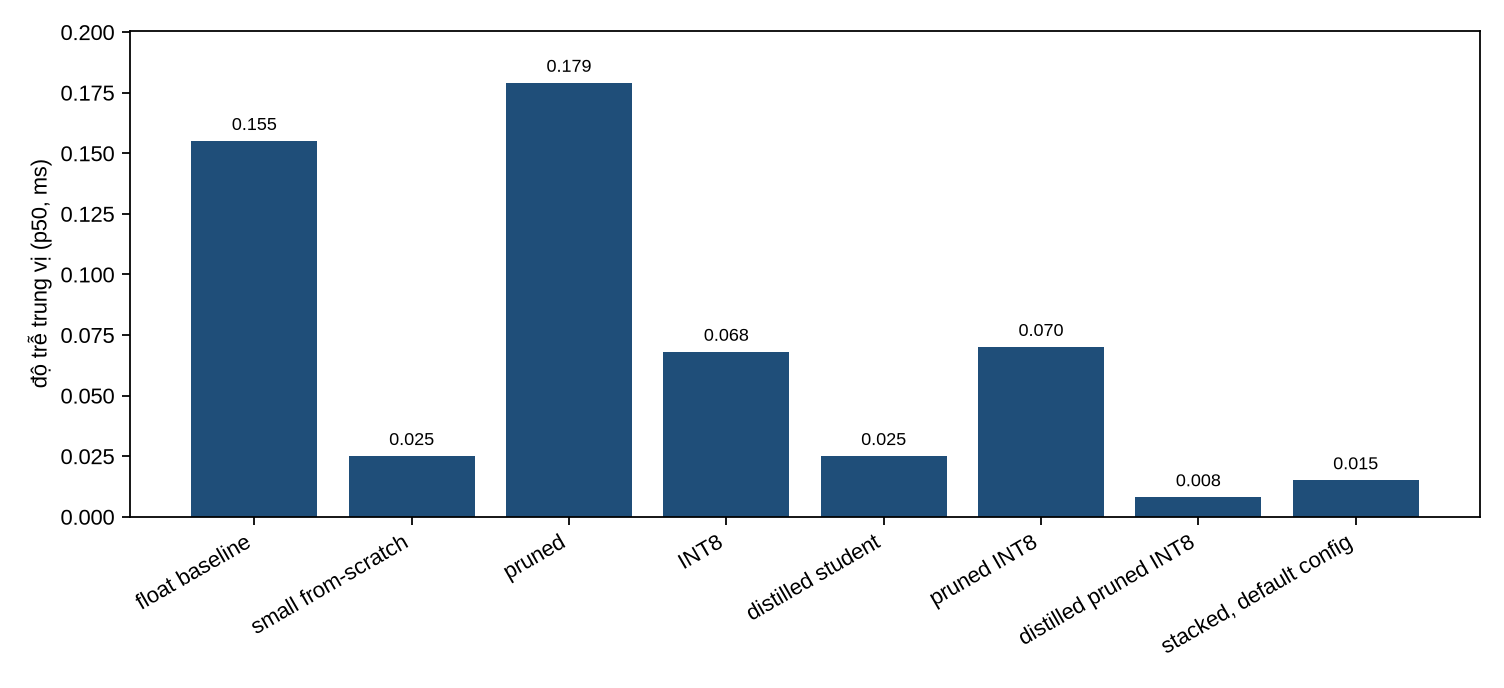
\includegraphics[width=0.88\textwidth]{figures/p50.png}}

Hình~\ref{fig:rawgzip} đặt kích thước thô cạnh gzip của cùng một dòng.
Hai cột xanh của float baseline và pruned cùng cao 1690.108 KB.
Cột cam của pruned chỉ còn 622.146 KB, nên phần cắt 60.31 phần trăm nằm ở gzip.
Phần cắt thô của dòng này là 0.00 phần trăm, và đó là lý do cột Kết quả ghi FAIL (raw).
Hai học sinh có cột thô trùng nhau ở 415.612 KB.
INT8 và pruned INT8 có cùng cột thô 431.992 KB, nhưng gzip của pruned INT8 còn 181.994 KB, thấp hơn 383.123 KB của INT8 một mình.
Hai dòng xếp có cùng cột thô 111.424 KB.
Gzip của cấu hình mặc định là 49.483 KB, và gzip của lần đã chỉnh là 87.025 KB.

\figframe{Kích thước tệp .tflite (KB, cột xanh) và kích thước tệp .tflite sau nén gzip mức 9, mốc thời gian 0 (KB, cột cam) của float baseline, small from-scratch, pruned, INT8, distilled student, pruned INT8, distilled pruned INT8 và stacked, default config.\label{fig:rawgzip}}{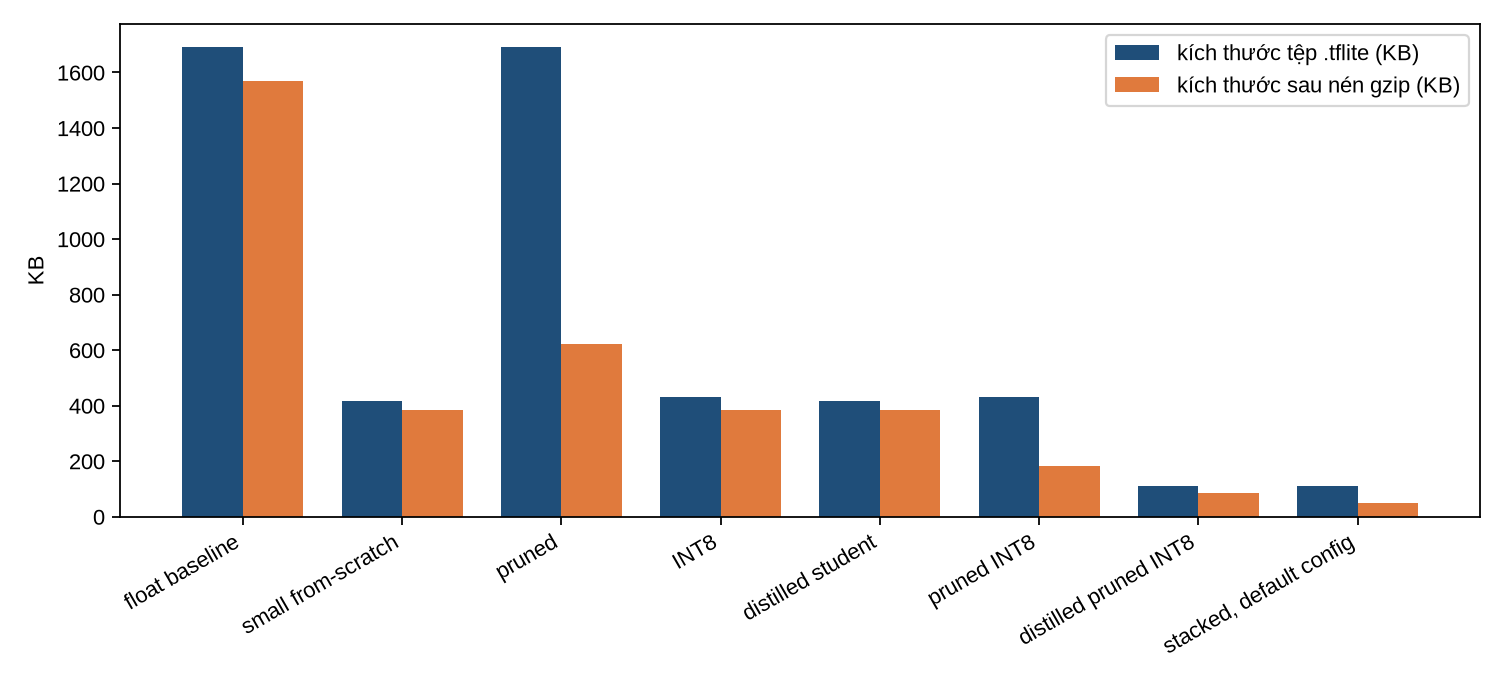
\includegraphics[width=0.88\textwidth]{figures/raw_vs_gzip.png}}

Hình~\ref{fig:p95} là đuôi độ trễ, không phải p50.
Pruning trên mô hình gốc có p95 bằng 0.261 ms, cao hơn 0.226 ms của mô hình gốc, cùng chiều với p50.
INT8 một mình còn 0.079 ms.
Pruned INT8 còn 0.094 ms, sát p50 0.070 ms của chính dòng đó.
Dòng đã chỉnh có p50 0.008 ms và p95 0.009 ms.
Cả hai số này thấp nhất trong tám dòng.
Cấu hình mặc định có p50 0.015 ms và p95 0.028 ms.

\figframe{Độ trễ phân vị 95 (p95, mili giây) của mỗi mô hình khi suy luận một ảnh kiểm tra trên CPU (batch = 1, một luồng; trung vị của ba lần đo): float baseline, small from-scratch, pruned, INT8, distilled student, pruned INT8, distilled pruned INT8 và stacked, default config. Giá trị lấy từ lần đo đã chốt.\label{fig:p95}}{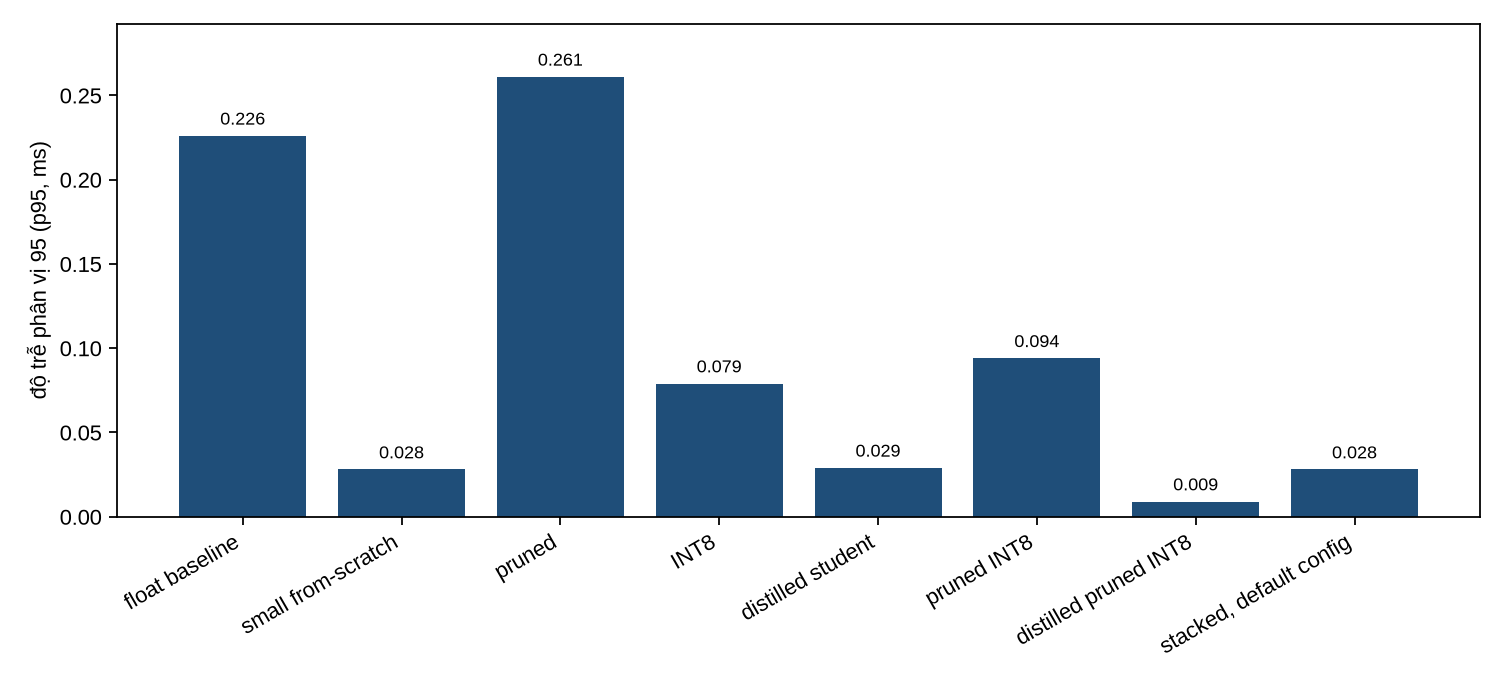
\includegraphics[width=0.88\textwidth]{figures/p95.png}}

Hình~\ref{fig:mem} là bộ nhớ đỉnh sau khi đã trừ sàn.
Pruning float là cột cao nhất, 7244 kB, trên cả 7108 kB của mô hình gốc.
INT8, hai học sinh và pruned INT8 nằm sát nhau: 4684 kB, 4692 kB, 4636 kB và 4648 kB.
Dòng đã chỉnh là cột thấp nhất, 4012 kB.
Cấu hình mặc định là 4016 kB.
Cùng một cách trừ sàn, thứ tự này so được giữa tám dòng.

\figframe{Bộ nhớ đỉnh (đỉnh bộ nhớ thường trú, VmHWM trừ tiến trình rỗng, kB) của float baseline, small from-scratch, pruned, INT8, distilled student, pruned INT8, distilled pruned INT8 và stacked, default config. Mỗi giá trị là trung vị của ba tiến trình có mô hình trừ trung vị của ba tiến trình rỗng.\label{fig:mem}}{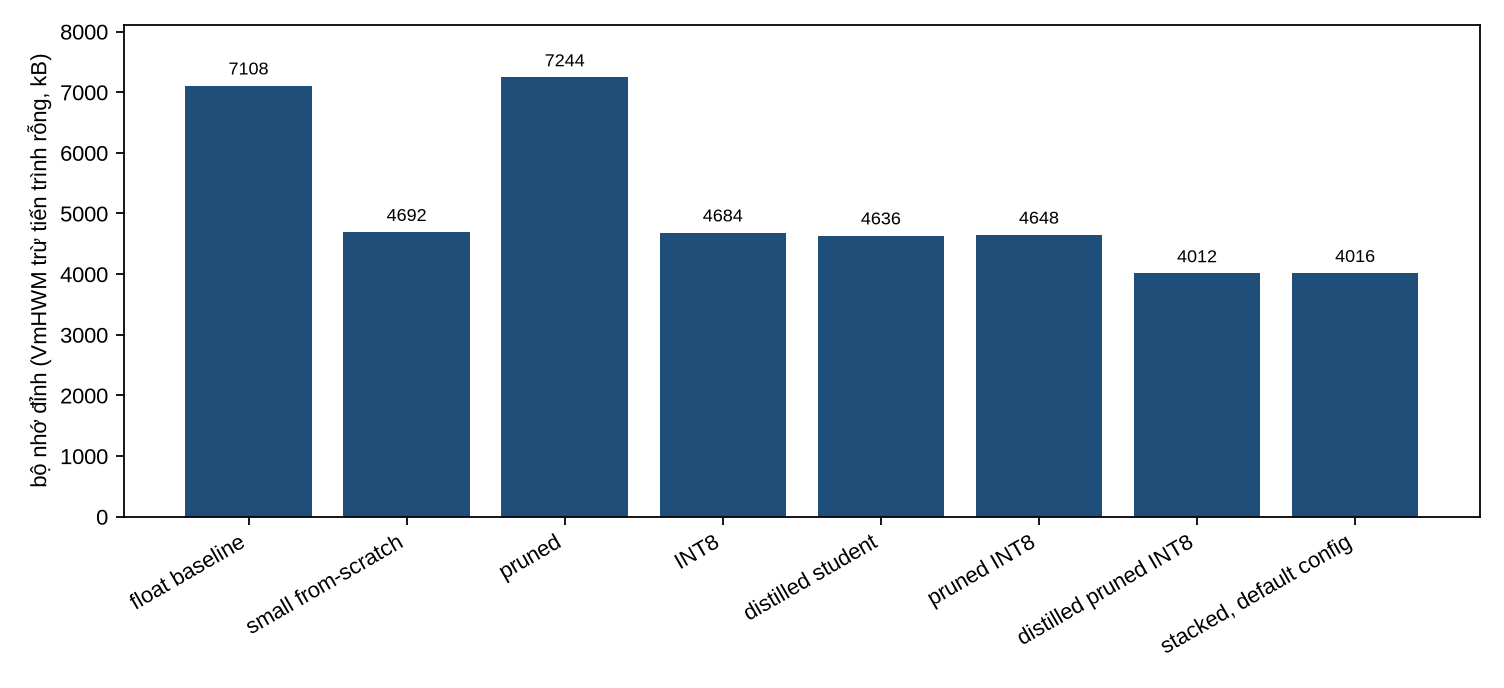
\includegraphics[width=0.88\textwidth]{figures/peak_mem.png}}

Ba hình kế tiếp lấy từ lần xem từng trọng số và từng ảnh, không phải từ tám file đã đo.
Hình~\ref{fig:hist} chỉ minh họa việc đưa trọng số nhỏ về không trên một bản sao của lớp tích chập đầu.
Hình đó không phải dòng pruned của Bảng~\ref{tab:results}.
Hình~\ref{fig:int8-scatter} và Hình~\ref{fig:int8-err} là cùng bản sao đó, với một thang demo cho riêng tensor này.
Điểm nằm gần đường chéo là trọng số được dựng lại gần giá trị float.
Độ lệch \(S(q-Z)-r\) trên histogram nằm quanh không.
Thang này không phải thang lưu trong file INT8, và hai hình không phải dòng INT8 của bảng.
Độ giảm 0.08 pp của dòng INT8 vẫn là số của bảng, không đọc ra từ histogram.
Hình~\ref{fig:distill-bars} là xác suất của mô hình gốc trên ảnh huấn luyện đầu, tại \(T=1\) và tại \(T=4\).
\(T=4\) làm đỉnh thấp đi và đẩy khối lượng sang lớp lân cận.
Ảnh này không phải ví dụ ba lớp ở Mục~\ref{sec:theory}, và không phải độ chính xác 0.9011 của học sinh.

\figframe{Minh họa pruning theo độ lớn trên một bản sao của lớp tích chập đầu: các trọng số nhỏ bị đặt về không. Bản sao này không phải mô hình pruned trong Bảng~\ref{tab:results}.\label{fig:hist}}{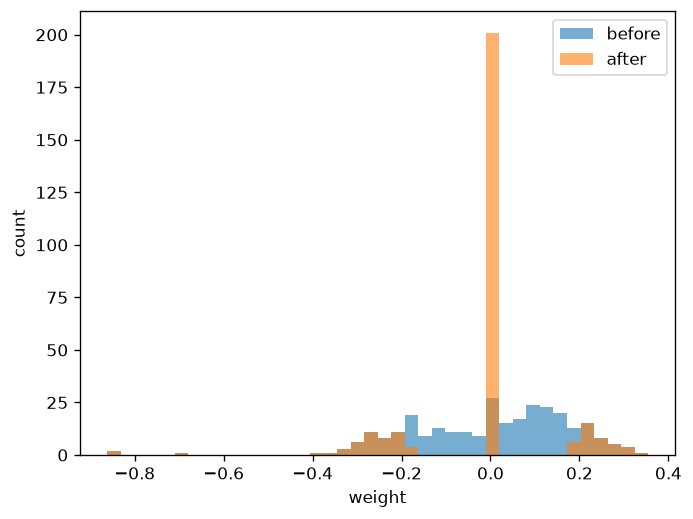
\includegraphics[width=0.72\textwidth]{figures/prune_hist.png}}

\figframe{Một lớp tích chập đầu của bản sao mô hình gốc: trục ngang là trọng số float \(r\), trục dọc là giá trị dựng lại \(S(q-Z)\). Thang demo của tensor này không phải thang trong file INT8, và hình không phải mô hình INT8 của Bảng~\ref{tab:results}.\label{fig:int8-scatter}}{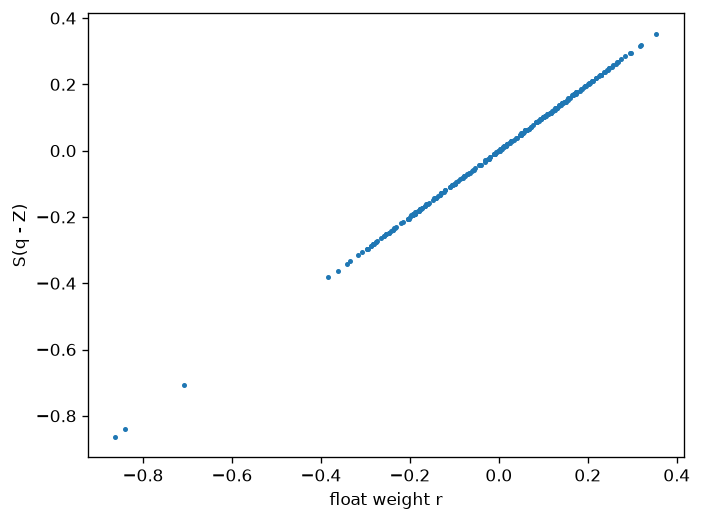
\includegraphics[width=0.72\textwidth]{figures/v3_int8_scatter.png}}

\figframe{Sai số dựng lại \(S(q-Z)-r\) trên cùng tensor với Hình~\ref{fig:int8-scatter}. Histogram này không phải độ giảm 0.08 pp của mô hình INT8.\label{fig:int8-err}}{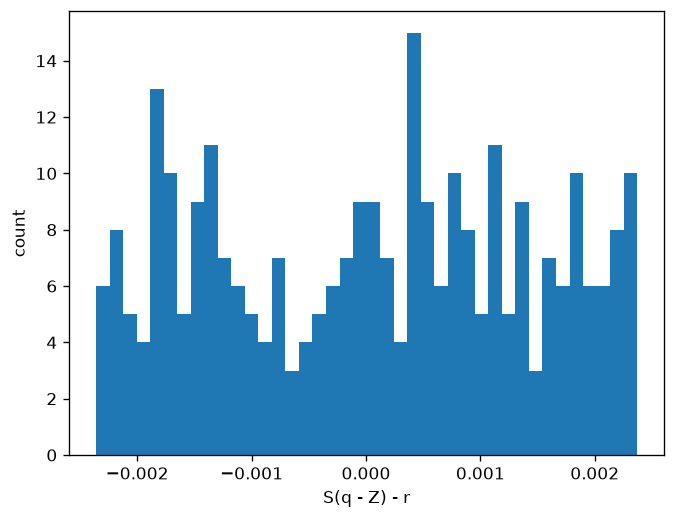
\includegraphics[width=0.72\textwidth]{figures/v3_int8_error_hist.png}}

\figframe{Xác suất của mô hình gốc trên ảnh huấn luyện đầu, tại \(T=1\) và \(T=4\). Hình này không phải ví dụ ba lớp, và không phải mô hình distilled student của Bảng~\ref{tab:results}.\label{fig:distill-bars}}{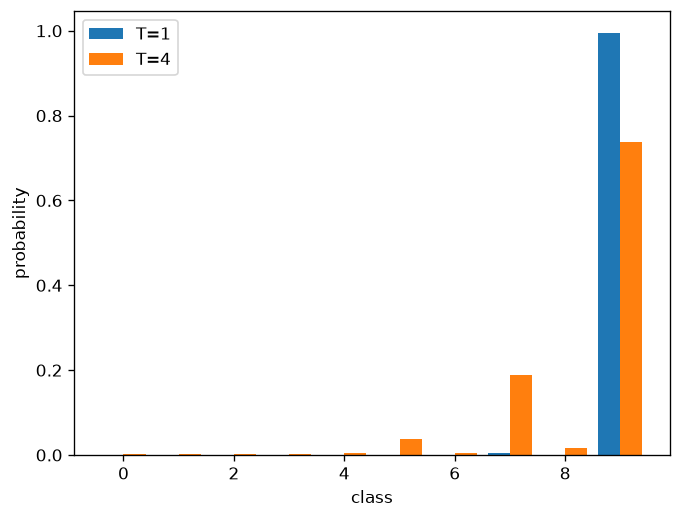
\includegraphics[width=0.72\textwidth]{figures/v3_distill_bars.png}}

\section{Phân tích độ nhạy siêu tham số}
\label{sec:sweep}

Mục này đổi một nút mỗi lần chạy.
Các nút còn lại giữ giá trị đã chốt.
Pruning giữ \(s_f=0.70\), 4 epoch, PolynomialDecay với power 3 và frequency 100, mọi lớp, Adam \(10^{-4}\), nhãn cứng, batch 128.
Distillation giữ \(T=4\), \(\alpha=0.5\), 8 kênh tích chập, dense 128, 10 epoch, learning rate \(10^{-3}\), và giữ epoch validation tốt nhất.
INT8 giữ full-integer, per-channel bật, 300 ảnh hiệu chuẩn đầu của tập huấn luyện.
Seed là 42.
Tập kiểm tra 10{,}000 ảnh không được dùng để chọn epoch.
Lần quét không đo p50, p95 hay bộ nhớ đỉnh.
Ba cột đó chỉ có trong Bảng~\ref{tab:results}.

Ngưỡng WITHIN NOISE của accuracy là \(\max\)(độ nhiễu anchor, \(2\times\) độ lệch chuẩn mẫu của tâm distilled trên năm seed, \(0.0010\)).
Độ nhiễu anchor là trị tuyệt đối của hiệu accuracy giữa lần chạy lại tại giá trị đã chốt và dòng tương ứng trong bảng đã chốt.
Pruning và INT8 chạy lại đúng 0.9099 và 0.9150, nên độ nhiễu anchor của hai phép đó là 0.
Distillation chạy lại được 0.8996, bảng đã chốt là 0.9011, nên độ nhiễu anchor là 0.0015.
Độ lệch chuẩn mẫu của tâm distilled là 0.001779, nên \(2\times 0.001779 = 0.003558\).
Ngưỡng dùng cho cả ba phép là 0.003558.
Một lệch accuracy nhỏ hơn hoặc bằng ngưỡng được ghi WITHIN NOISE khi dự đoán là một hướng.
Gzip được gọi là đi ngang khi lệch không quá 5 KB.

\subsection{Pruning}

\(s_f\) là phần trọng số bị đưa về không ở cuối lịch \cite{zhu2017}.
Tăng \(s_f\) bỏ nhiều trọng số nhỏ hơn, nên accuracy được dự đoán giảm và gzip của file float được dự đoán giảm.
Số epoch là thời gian để các trọng số còn lại hồi lại trong lúc độ thưa đi từ 0 lên \(s_f\).
Accuracy được dự đoán tăng rồi đi ngang.
Gzip được dự đoán đi ngang, vì \(s_f\) cuối không đổi.
PolynomialDecay nâng độ thưa dần.
ConstantSparsity đặt đúng \(s_f\) từ bước 0.
Accuracy của ConstantSparsity được dự đoán thấp hơn.
Hai lịch kết thúc cùng \(s_f\), nên gzip phải khớp trong vài KB.
Lệch lớn hơn mức đó là dấu hiệu lỗi.
Nút lớp chọn mọi lớp, hoặc chỉ các lớp dense.
Phần dense chiếm gần hết tham số, nên dense-only được dự đoán giữ accuracy cao hơn một chút và gzip lớn hơn một chút.

Lớp tích chập của mô hình gốc có 18{,}816 tham số, trong đó 18{,}720 là kernel và 96 là bias.
Các lớp dense có 402{,}826 tham số, trong đó 402{,}688 là kernel và 138 là bias.
Dense chiếm \(402826/421642\), tức 95.5 phần trăm số tham số.
Vì vậy bỏ pruning trên các lớp tích chập chỉ chừa lại một phần nhỏ các số khác không.

\begin{table}[H]
\centering
\caption{Pruning trên float baseline, dự đoán so với lần đo khi đổi một nút, với mốc \(s_f=0.70\), 4 epoch, PolynomialDecay, mọi lớp. Accuracy là độ chính xác trên tập kiểm tra (10{,}000 ảnh) và gzip là kích thước tệp .tflite sau nén gzip (KB).}
\label{tab:sweep-prune}
\footnotesize
\begin{tabular}{|l|l|l|l|r|r|l|}
\hline
Nút & Giá trị & Dự đoán acc. & Dự đoán gzip & Acc. & Gzip KB & Kết luận \\ \hline
\(s_f\) & 0.50 & cao hơn mốc & lớn hơn mốc & 0.9178 & 925.305 & CONFIRMED \\ \hline
\(s_f\) & 0.70 & mốc & mốc & 0.9099 & 622.146 & mốc \\ \hline
\(s_f\) & 0.80 & thấp hơn mốc & nhỏ hơn mốc & 0.8945 & 458.779 & CONFIRMED \\ \hline
\(s_f\) & 0.90 & thấp hơn mốc & nhỏ hơn mốc & 0.8149 & 279.680 & CONFIRMED \\ \hline
epochs & 1 & thấp hơn mốc & đi ngang & 0.9031 & 618.839 & CONFIRMED \\ \hline
epochs & 4 & mốc & mốc & 0.9099 & 622.146 & mốc \\ \hline
epochs & 8 & không thấp hơn & đi ngang & 0.9141 & 620.965 & CONFIRMED \\ \hline
schedule & PolynomialDecay & mốc & mốc & 0.9099 & 622.146 & mốc \\ \hline
schedule & ConstantSparsity & thấp hơn mốc & đi ngang & 0.9097 & 622.564 & WITHIN NOISE \\ \hline
layers & all & mốc & mốc & 0.9099 & 622.146 & mốc \\ \hline
layers & dense-only & cao hơn mốc & lớn hơn mốc & 0.9167 & 663.939 & CONFIRMED \\ \hline
\end{tabular}
\end{table}

Bốn giá trị \(s_f\) đi đúng hướng đã dự đoán.
Từ 0.50 lên 0.90, accuracy đi từ 0.9178 xuống 0.8149 và gzip đi từ 925.305 KB xuống 279.680 KB.
Một epoch cho 0.9031.
Tám epoch cho 0.9141.
Gzip của ba mốc epoch là 618.839 KB, 622.146 KB và 620.965 KB, đều trong 5 KB.
ConstantSparsity đạt 0.9097, thấp hơn mốc 0.0002.
Mức 0.0002 nằm dưới ngưỡng 0.003558, nên dòng là WITHIN NOISE.
Gzip là 622.564 KB, cao hơn mốc 0.418 KB.
Mức đó nằm trong vài KB, nên không phải lỗi lệch lịch.
Dense-only đạt 0.9167 và gzip 663.939 KB, cao hơn mốc 41.793 KB, đúng với phần kernel tích chập còn dày.

\figframe{Độ chính xác trên tập kiểm tra và kích thước tệp .tflite sau nén gzip (KB) theo độ thưa cuối \(s_f\) của pruning. Vạch đứt và vòng tròn hở là giá trị đã chốt \(0.70\).\label{fig:sweep-sf}}{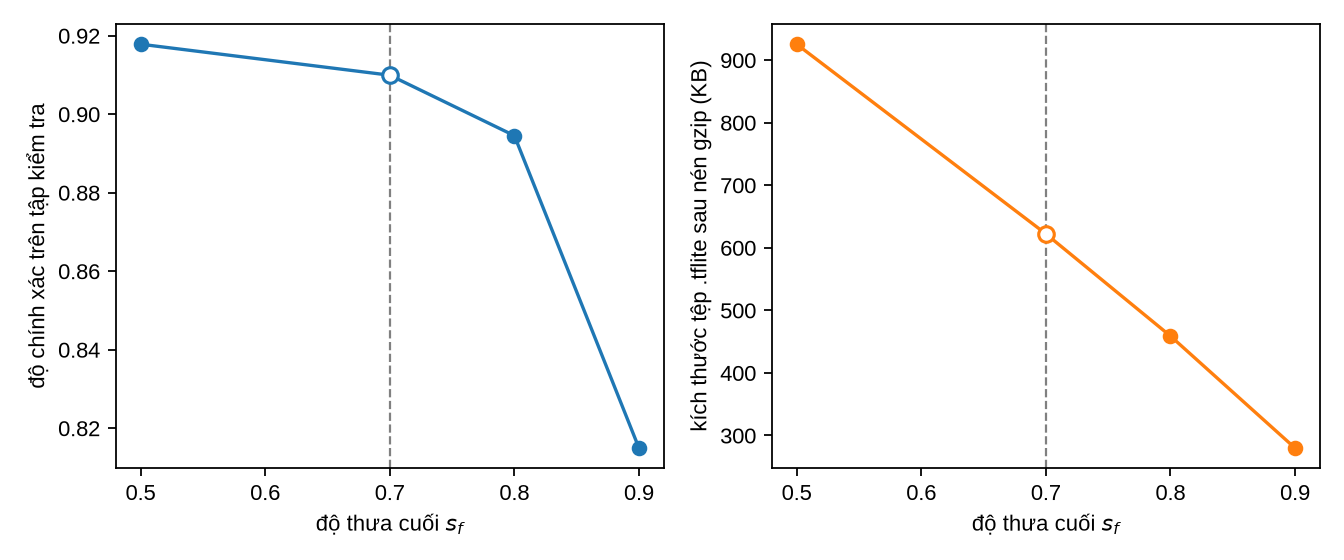
\includegraphics[width=0.88\textwidth]{figures/sweep_prune_sf.png}}

\figframe{Độ chính xác trên tập kiểm tra và kích thước tệp .tflite sau nén gzip (KB) theo số epoch pruning. Vạch đứt là 4 epoch và \(s_f\) cuối vẫn là 0.70.\label{fig:sweep-prune-ep}}{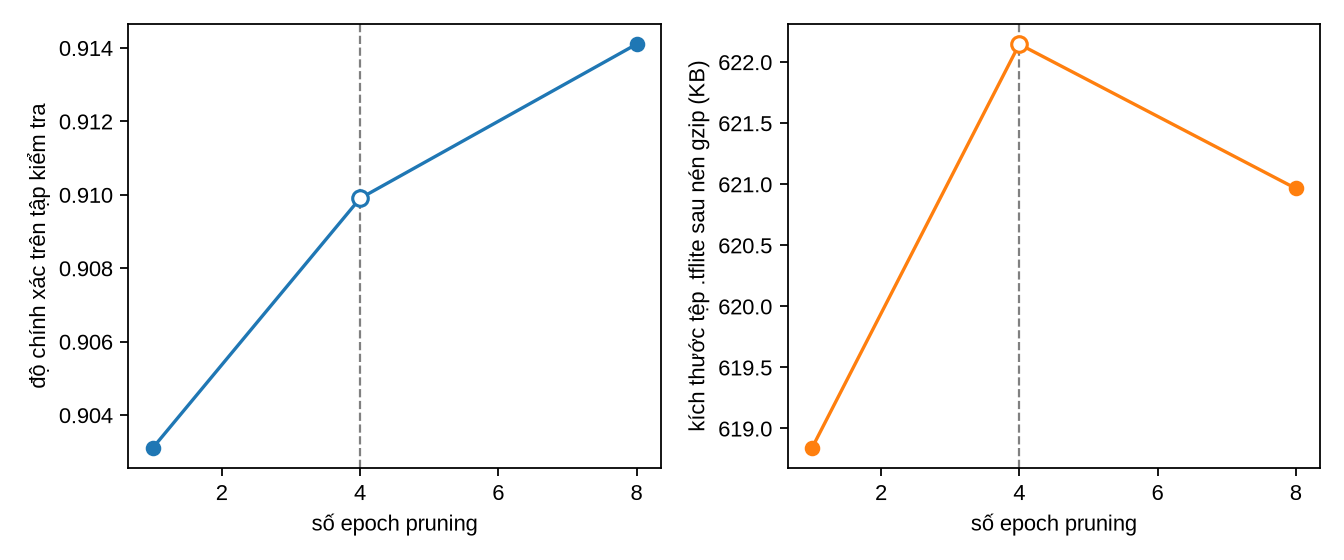
\includegraphics[width=0.88\textwidth]{figures/sweep_prune_epochs.png}}

\subsection{Distillation}

\(T\) làm mềm phân phối của giáo viên trước khi so với học sinh \cite{hinton2015}.
Dự đoán là accuracy tăng từ \(T=1\) tới \(T=4\), rồi giảm ở \(T=8\).
\(\alpha\) là trọng số của phần mềm.
\(\alpha=0\) là nhãn cứng.
Dự đoán là accuracy tăng từ 0 tới 0.5, rồi đi ngang hoặc giảm nhẹ ở 0.9.
Số epoch là ngân sách để chọn epoch validation tốt nhất.
Năm epoch được dự đoán thấp hơn 10 epoch.
Hai mươi epoch được dự đoán đi ngang, vì epoch tốt có thể đã nằm trong 10 epoch đầu.
Learning rate \(10^{-4}\) và \(10^{-2}\) được dự đoán thấp hơn \(10^{-3}\).
Đây là hành vi tối ưu tổng quát, kiểm tra bằng thực nghiệm, không lấy từ một bài báo của phương pháp.
Bốn nút này không đổi kiến trúc, nên gzip được dự đoán đi ngang.
Số kênh và số đơn vị dense đổi kích thước lớp dense sau flatten.
Cả accuracy và gzip được dự đoán tăng theo độ rộng, với cả nhãn mềm và nhãn cứng.

\begin{table}[H]
\centering
\caption{Distillation khi đổi một nút và giữ độ rộng, với mốc \(T=4\), \(\alpha=0.5\), 10 epoch, learning rate \(10^{-3}\). Accuracy là độ chính xác trên tập kiểm tra và gzip là kích thước tệp .tflite sau nén gzip (KB).}
\label{tab:sweep-distill}
\footnotesize
\begin{tabular}{|l|l|l|l|r|r|l|}
\hline
Nút & Giá trị & Dự đoán acc. & Dự đoán gzip & Acc. & Gzip KB & Kết luận \\ \hline
\(T\) & 1 & thấp hơn mốc & đi ngang & 0.9055 & 383.941 & REFUTED \\ \hline
\(T\) & 2 & thấp hơn mốc & đi ngang & 0.8992 & 383.925 & WITHIN NOISE \\ \hline
\(T\) & 4 & mốc & mốc & 0.8996 & 384.081 & mốc \\ \hline
\(T\) & 8 & thấp hơn mốc & đi ngang & 0.8986 & 384.067 & WITHIN NOISE \\ \hline
\(\alpha\) & 0 & thấp hơn mốc & đi ngang & 0.9022 & 384.165 & WITHIN NOISE \\ \hline
\(\alpha\) & 0.1 & thấp hơn mốc & đi ngang & 0.8993 & 383.908 & WITHIN NOISE \\ \hline
\(\alpha\) & 0.5 & mốc & mốc & 0.8996 & 384.081 & mốc \\ \hline
\(\alpha\) & 0.9 & đi ngang hoặc thấp hơn & đi ngang & 0.8960 & 384.129 & CONFIRMED \\ \hline
epochs & 5 & thấp hơn mốc & đi ngang & 0.8883 & 383.392 & CONFIRMED \\ \hline
epochs & 10 & mốc & mốc & 0.8996 & 384.081 & mốc \\ \hline
epochs & 20 & đi ngang & đi ngang & 0.9056 & 384.368 & REFUTED \\ \hline
learning rate & \(10^{-4}\) & thấp hơn mốc & đi ngang & 0.8526 & 381.908 & CONFIRMED \\ \hline
learning rate & \(10^{-3}\) & mốc & mốc & 0.8996 & 384.081 & mốc \\ \hline
learning rate & \(10^{-2}\) & thấp hơn mốc & đi ngang & 0.8999 & 385.348 & WITHIN NOISE \\ \hline
\end{tabular}
\end{table}

Trên năm seed, \(T=1\) đạt \(0.9033 \pm 0.0022\), còn \(T=4\) đạt \(0.8982 \pm 0.0018\), hiệu \(+0.0051\).
\(T=1\) cũng cao hơn hard-label \(\alpha=0\), với \(0.9033\) so với \(0.8991\).
Dự đoán \(T=1\) thấp hơn \(T=4\) vẫn bị REFUTED.
\(T=2\) và \(T=8\) lệch \(-0.0004\) và \(-0.0010\), đều trong ngưỡng.
\(\alpha=0\) đạt 0.9022, cao hơn mốc 0.0026.
Mức 0.0026 nhỏ hơn 0.003558, nên dòng là WITHIN NOISE.
\(\alpha=0.9\) giảm xuống 0.8960, đúng phía đã dự đoán.
Năm epoch còn 0.8883.
Hai mươi epoch lên 0.9056, lệch \(+0.0060\), nên dự đoán đi ngang bị REFUTED.
Learning rate \(10^{-4}\) rơi xuống 0.8526.
Learning rate \(10^{-2}\) là 0.8999, lệch \(+0.0003\), trong ngưỡng.
Gzip của cả bảng này nằm trong khoảng 381.908 KB đến 385.348 KB.

Năm seed 42, 43, 44, 45 và 46 dùng lần chạy đầu của seed 42.
Tâm distilled có accuracy trung bình \(0.8982 \pm 0.0018\).
Tâm hard-label có \(0.8991 \pm 0.0047\).
\(T=1\) có \(0.9033 \pm 0.0022\).
Phần tăng distilled trừ hard-label trên từng seed là \(-0.0026\), \(+0.0007\), \(-0.0071\), \(+0.0011\) và \(+0.0034\).
Trung bình phần tăng là \(-0.0009 \pm 0.0041\).
Trị tuyệt đối của trung bình nhỏ hơn một độ lệch chuẩn, nên distillation không cho phần tăng đáng tin trong thiết lập này.
Chạy lại seed 42 cho accuracy 0.8985, 0.8990 và 0.9012 ở ba cấu hình đó.
Ba số này không trùng 0.8996, 0.9022 và 0.9055 của lần đầu.
Độ lệch chuẩn ở trên là độ lệch chuẩn mẫu của năm seed.

\figframe{Độ chính xác trên tập kiểm tra và kích thước tệp .tflite sau nén gzip (KB) theo nhiệt độ \(T\) của distillation. Vạch đứt là \(T=4\).\label{fig:sweep-T}}{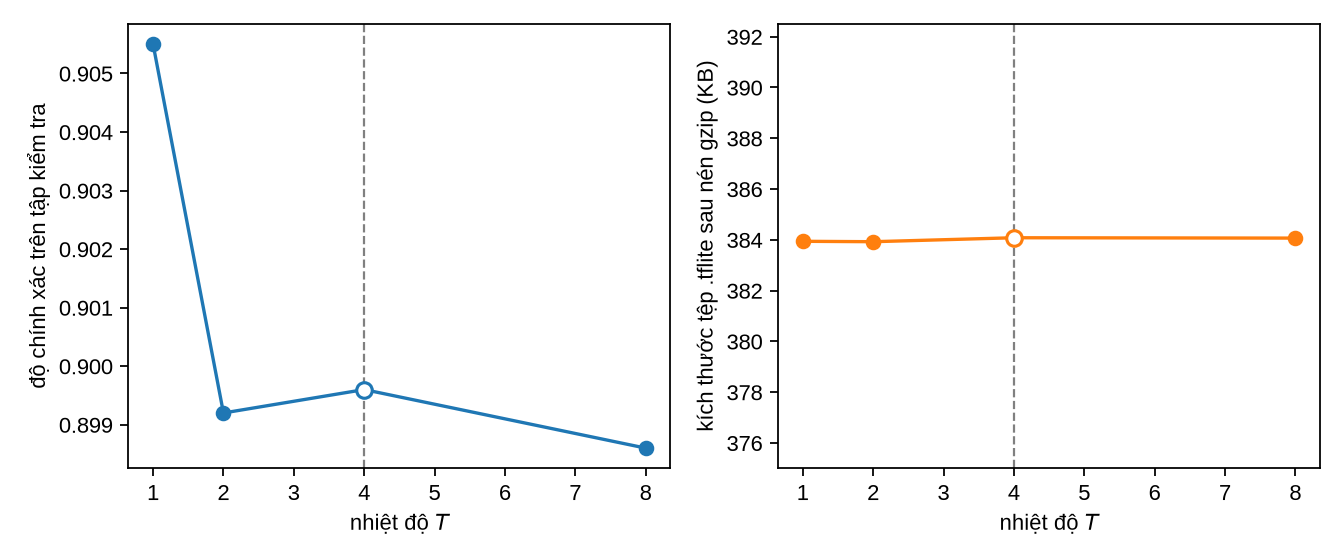
\includegraphics[width=0.88\textwidth]{figures/sweep_distill_T.png}}

\figframe{Độ chính xác trên tập kiểm tra và kích thước tệp .tflite sau nén gzip (KB) theo \(\alpha\) của distillation. Vạch đứt là \(\alpha=0.5\) và giá trị 0 là nhãn cứng.\label{fig:sweep-alpha}}{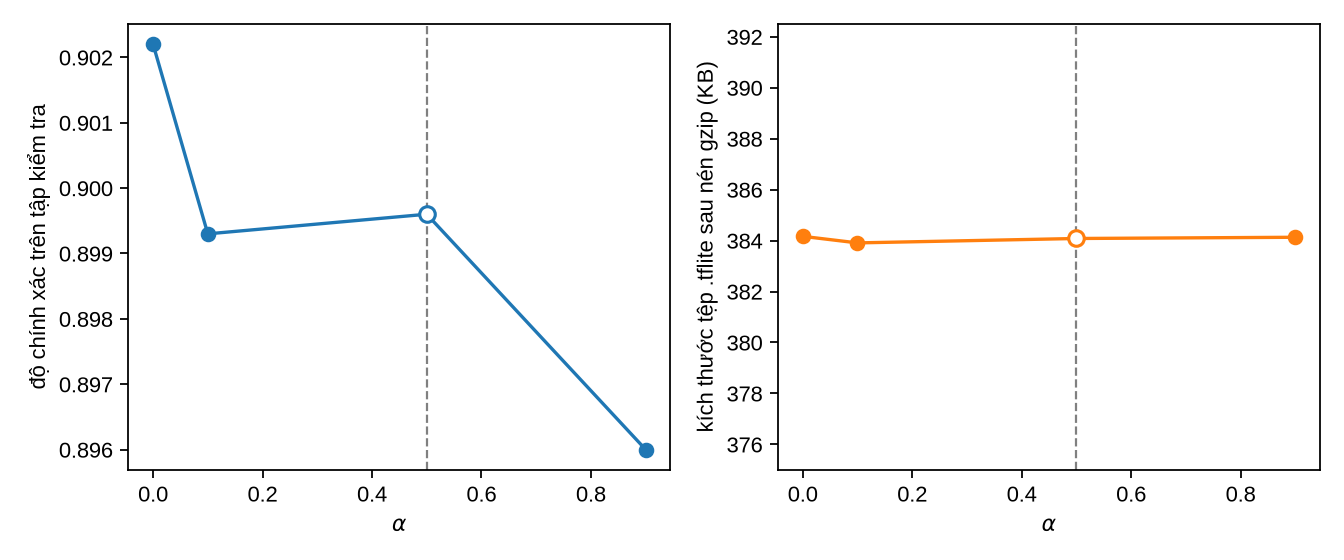
\includegraphics[width=0.88\textwidth]{figures/sweep_distill_alpha.png}}

\figframe{Độ chính xác trên tập kiểm tra và kích thước tệp .tflite sau nén gzip (KB) theo số epoch distillation. Vạch đứt là 10 epoch.\label{fig:sweep-distill-ep}}{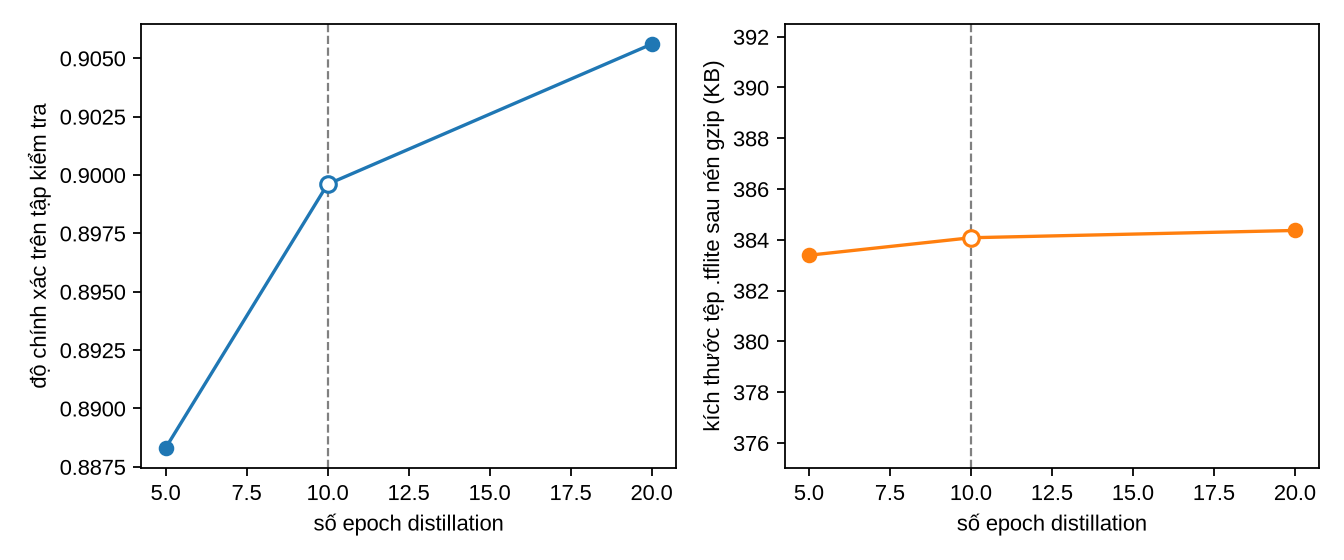
\includegraphics[width=0.88\textwidth]{figures/sweep_distill_epochs.png}}

\figframe{Độ chính xác trên tập kiểm tra và kích thước tệp .tflite sau nén gzip (KB) theo learning rate của distillation. Trục ngang là thang log và vạch đứt là \(10^{-3}\).\label{fig:sweep-lr}}{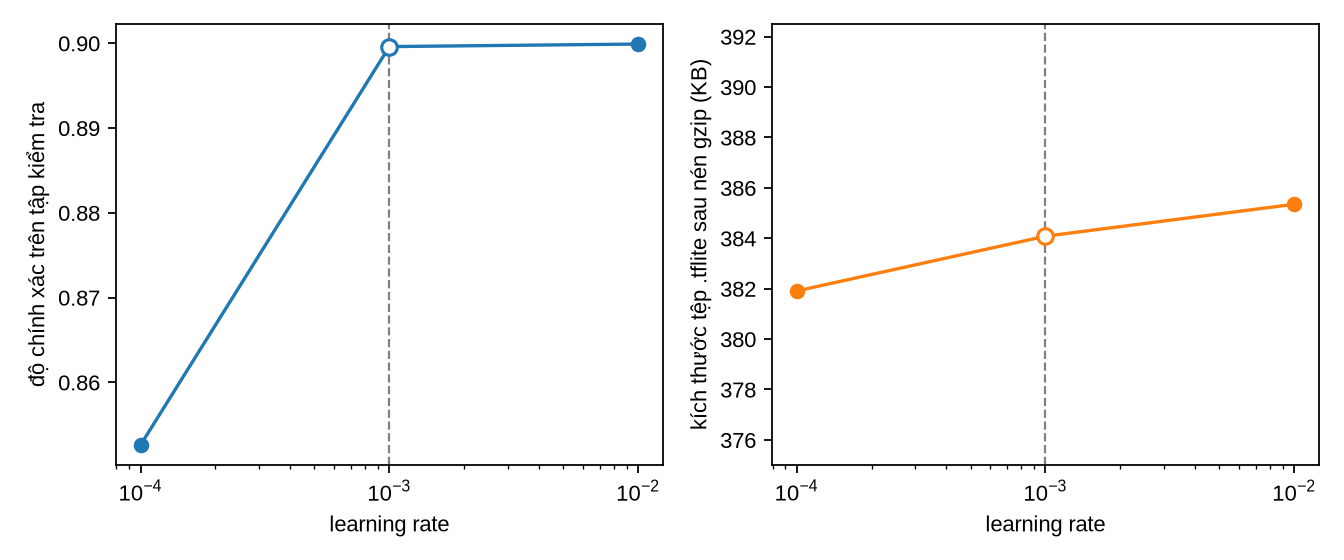
\includegraphics[width=0.88\textwidth]{figures/sweep_distill_lr.png}}

\begin{table}[H]
\centering
\caption{Độ rộng học sinh. Mỗi độ rộng có distilled (\(\alpha=0.5\)) và hard-label (\(\alpha=0\)). Mốc độ rộng là 8 kênh và dense 128.}
\label{tab:sweep-width}
\footnotesize
\begin{tabular}{|l|l|l|l|r|r|l|}
\hline
Nút & Giá trị & Dự đoán acc. & Dự đoán gzip & Acc. & Gzip KB & Kết luận \\ \hline
filters, distilled & 4 & thấp hơn 8 & nhỏ hơn 8 & 0.8839 & 194.474 & CONFIRMED \\ \hline
filters, distilled & 8 & mốc & mốc & 0.8996 & 384.081 & mốc \\ \hline
filters, distilled & 16 & cao hơn 8 & lớn hơn 8 & 0.8996 & 770.085 & WITHIN NOISE \\ \hline
filters, hard-label & 4 & thấp hơn 8 & nhỏ hơn 8 & 0.8916 & 194.586 & CONFIRMED \\ \hline
filters, hard-label & 8 & mốc nhánh & mốc nhánh & 0.9022 & 384.165 & mốc nhánh \\ \hline
filters, hard-label & 16 & cao hơn 8 & lớn hơn 8 & 0.9075 & 770.542 & CONFIRMED \\ \hline
dense, distilled & 64 & thấp hơn 128 & nhỏ hơn 128 & 0.8905 & 195.192 & CONFIRMED \\ \hline
dense, distilled & 128 & mốc & mốc & 0.8996 & 384.081 & mốc \\ \hline
dense, distilled & 256 & cao hơn 128 & lớn hơn 128 & 0.9062 & 761.432 & CONFIRMED \\ \hline
dense, hard-label & 64 & thấp hơn 128 & nhỏ hơn 128 & 0.8954 & 195.321 & CONFIRMED \\ \hline
dense, hard-label & 128 & mốc nhánh & mốc nhánh & 0.9022 & 384.165 & mốc nhánh \\ \hline
dense, hard-label & 256 & cao hơn 128 & lớn hơn 128 & 0.9028 & 761.806 & WITHIN NOISE \\ \hline
\end{tabular}
\end{table}

Phần tăng từ distillation tại một độ rộng là accuracy distilled trừ accuracy hard-label cùng độ rộng.
Tại 4 kênh, hiệu là \(0.8839-0.8916=-0.0077\).
Tại 16 kênh, hiệu là \(0.8996-0.9075=-0.0079\).
Hiệu của hai hiệu này là 0.0002, nhỏ hơn ngưỡng 0.003558, nên WITHIN NOISE.
Tại dense 64, hiệu là \(0.8905-0.8954=-0.0049\).
Tại dense 256, hiệu là \(0.9062-0.9028=+0.0034\).
Độ rộng lớn hơn lại là phía có phần tăng dương, ngược với dự đoán phần tăng sẽ lớn hơn ở học sinh hẹp, nên dòng này REFUTED.
Tại chính độ rộng đã chốt, hiệu là \(0.8996-0.9022=-0.0026\).
Số 0.37 pp của hai học sinh trong Bảng~\ref{tab:results} là một cặp file khác, không phải hiệu này.

\figframe{Độ chính xác trên tập kiểm tra và kích thước tệp .tflite sau nén gzip (KB) theo số kênh tích chập. Đường xanh là distilled (\(\alpha=0.5\)), đường cam là hard-label (\(\alpha=0\)), và vạch đứt là 8 kênh.\label{fig:sweep-filters}}{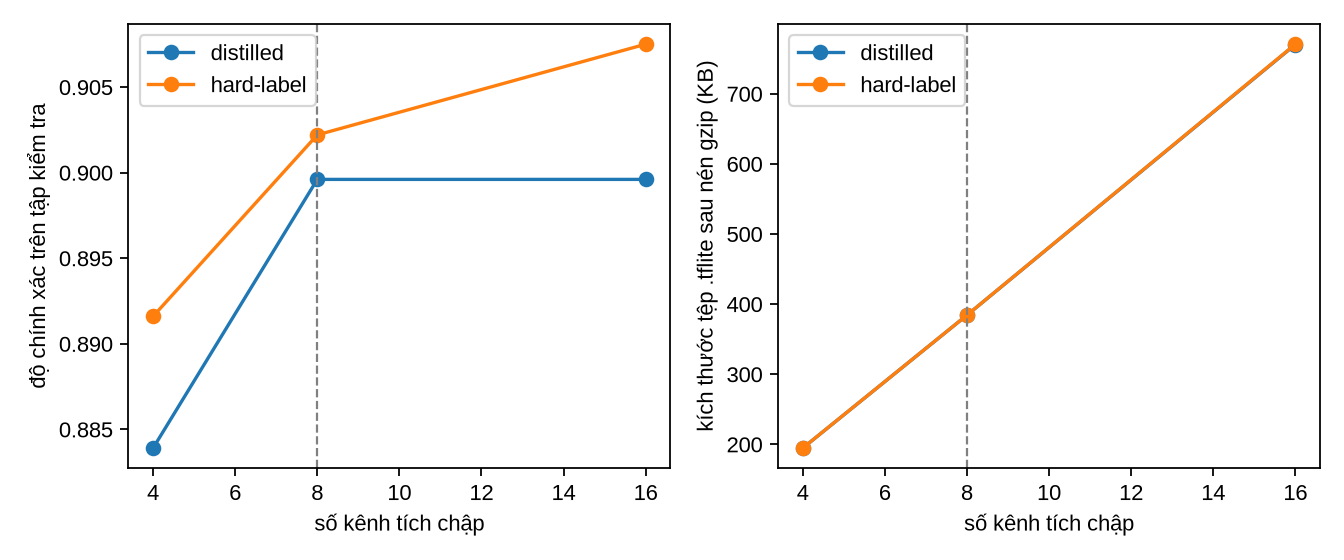
\includegraphics[width=0.88\textwidth]{figures/sweep_filters.png}}

\figframe{Độ chính xác trên tập kiểm tra và kích thước tệp .tflite sau nén gzip (KB) theo số đơn vị dense. Đường xanh là distilled (\(\alpha=0.5\)), đường cam là hard-label (\(\alpha=0\)), và vạch đứt là 128.\label{fig:sweep-dense}}{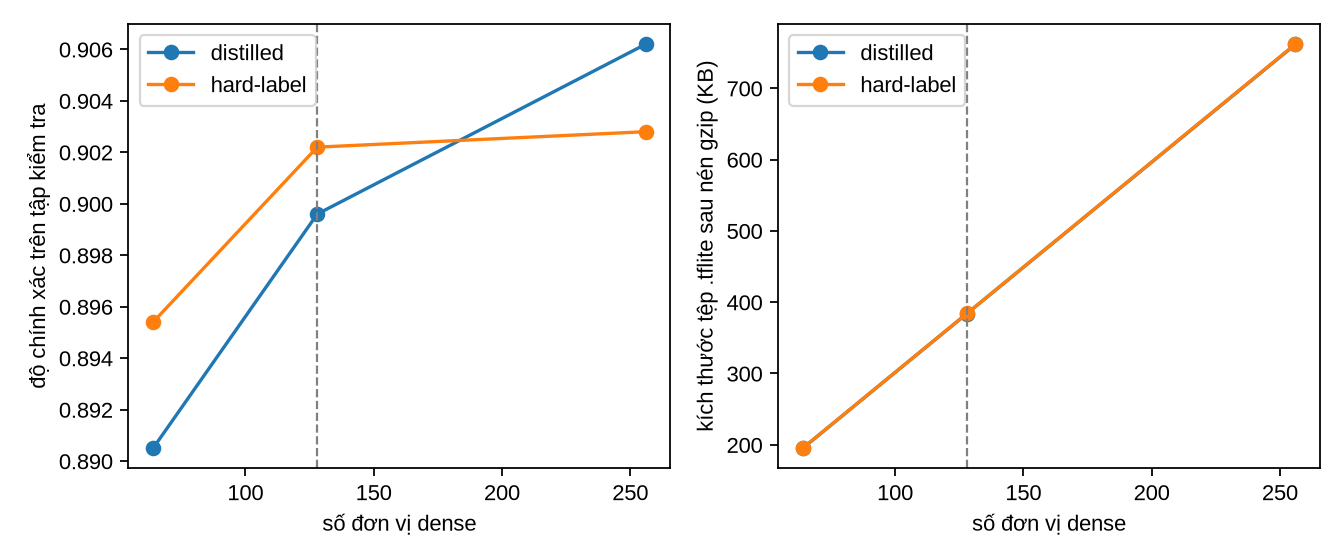
\includegraphics[width=0.88\textwidth]{figures/sweep_dense.png}}

\subsection{INT8}

Full-integer lượng tử hóa cả trọng số và activation \cite{jacob2018}.
Dynamic-range lượng tử hóa trọng số và giữ activation ở float.
Float16 giữ lưới 16 bit.
Accuracy được dự đoán tăng ở cả hai chế độ so với full-integer, và float16 cao hơn dynamic-range.
Gzip của float16 được dự đoán tăng mạnh.
Gzip của dynamic-range được dự đoán đi ngang.
Tắt per-channel dùng một scale cho cả lớp, nên accuracy được dự đoán giảm.
Các scale thêm được dự đoán chỉ chiếm vài byte, nên gzip đi ngang.
Số ảnh hiệu chuẩn ước lượng khoảng activation.
Từ 10 lên 300, accuracy được dự đoán tăng.
Từ 300 lên 1000, accuracy và gzip được dự đoán đi ngang.

\begin{table}[H]
\centering
\caption{INT8 trên float baseline. Mốc là full-integer, per-channel bật, 300 ảnh hiệu chuẩn. Accuracy là độ chính xác trên tập kiểm tra và gzip là kích thước tệp .tflite sau nén gzip (KB).}
\label{tab:sweep-int8}
\footnotesize
\begin{tabular}{|l|l|l|l|r|r|l|}
\hline
Nút & Giá trị & Dự đoán acc. & Dự đoán gzip & Acc. & Gzip KB & Kết luận \\ \hline
mode & full-int8 & mốc & mốc & 0.9150 & 383.123 & mốc \\ \hline
mode & dynamic-range & cao hơn mốc & đi ngang & 0.9158 & 383.433 & WITHIN NOISE \\ \hline
mode & float16 & cao hơn mốc & lớn hơn nhiều & 0.9160 & 782.081 & WITHIN NOISE \\ \hline
per-channel & on & mốc & mốc & 0.9150 & 383.123 & mốc \\ \hline
per-channel & off & thấp hơn mốc & đi ngang & 0.9149 & 310.928 & REFUTED \\ \hline
calibration & 10 & thấp hơn mốc & đi ngang & 0.9150 & 383.123 & WITHIN NOISE \\ \hline
calibration & 100 & thấp hơn mốc & đi ngang & 0.9150 & 383.123 & WITHIN NOISE \\ \hline
calibration & 300 & mốc & mốc & 0.9150 & 383.123 & mốc \\ \hline
calibration & 1000 & đi ngang & đi ngang & 0.9152 & 383.097 & CONFIRMED \\ \hline
\end{tabular}
\end{table}

Dynamic-range đạt 0.9158, lệch \(+0.0008\), trong ngưỡng 0.003558, và gzip cao hơn mốc 0.310 KB, nên dòng là WITHIN NOISE.
Float16 đạt 0.9160, lệch accuracy \(+0.0010\), cũng trong ngưỡng, dù gzip tăng 398.958 KB, nên dòng là WITHIN NOISE.
Tắt per-channel chỉ giảm accuracy 0.0001, nhưng gzip xuống 310.928 KB, thấp hơn 72.195 KB.
Phần gzip không đi ngang, nên cả dòng REFUTED.
File thô là 431.992 KB khi per-channel bật và 426.464 KB khi tắt.
Kernel dense có 401{,}408 mã int8.
Số mã khác nhau là 255 khi bật và 188 khi tắt.
Gzip giảm vì bảng mã hẹp hơn.
Bộ sinh representative dataset được gọi đủ 10, 100, 300 và 1000 ảnh.
Scale đầu vào của cả bốn file là 0.0039215689 và zero-point là \(-128\).
Scale đầu ra của lớp tích chập đầu là 0.0034249111 với 10 ảnh, 0.0035007943 với cả 100 và 300 ảnh, và 0.003533717 với 1000 ảnh.
File 100 ảnh và file 300 ảnh trùng nhau từng byte, nên thêm ảnh trong khoảng đó không đổi mô hình lượng tử.
Một nghìn ảnh lên 0.9152, lệch \(+0.0002\), và gzip 383.097 KB.
Lệch này nằm trong ngưỡng, và gzip lệch 0.026 KB, nên dự đoán đi ngang được ghi CONFIRMED.

\figframe{Độ chính xác trên tập kiểm tra và kích thước tệp .tflite sau nén gzip (KB) theo số ảnh hiệu chuẩn của INT8. Vạch đứt là 300 ảnh và thang dọc được nới để lệch cỡ một ảnh không thành một vách.\label{fig:sweep-cal}}{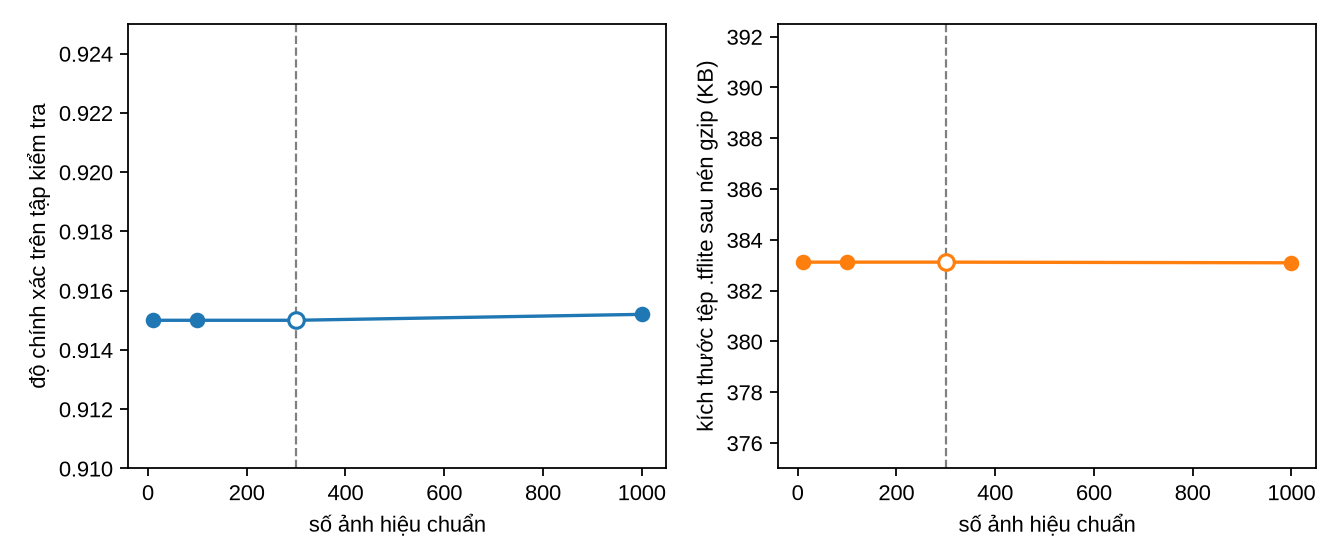
\includegraphics[width=0.88\textwidth]{figures/sweep_int8_cal.png}}

Lần quét một nút dùng một seed, trừ tâm distillation được lặp năm seed.
Tập ảnh là một tập Fashion-MNIST, và lần quét không có p50, p95 hay bộ nhớ đỉnh.
Trên 33 so sánh có hướng, 16 CONFIRMED, 4 REFUTED và 13 WITHIN NOISE.
Bốn dòng REFUTED là \(T=1\), 20 epoch, phần tăng theo dense, và per-channel tắt.

\section{Hạn chế và hướng tiếp}

Bảng~\ref{tab:results} đủ để chấm ba vạch trên Fashion-MNIST, và không đủ để kết luận ngoài phạm vi đó.
Mọi dòng dùng một tập ảnh và một lần chia 54{,}000, 6{,}000, 10{,}000.
Năm seed 42 đến 46 của tâm học sinh nằm ở Mục~\ref{sec:sweep}.
Một lần chạy lại seed 42 không tự lặp (0.8996 so với 0.8985 ở tâm distilled), nên huấn luyện không bit-deterministic trên thiết lập này, và độ lệch chuẩn của năm seed là khoảng bất định để đọc các lệch.
Độ trễ là một CPU, một luồng, một ảnh.
Máy đo dùng CPU 13th Gen Intel(R) Core(TM) i9-13900HX.
Vì vậy 0.008 ms hay 0.179 ms là thứ tự trên máy đo, chưa phải thứ tự trên một vi điều khiển hoặc một điện thoại.
Bộ nhớ đỉnh là hiệu \texttt{VmHWM} sau khi trừ sàn.
Sàn đo lại là 34944 kB, trung vị của 34932 kB, 34944 kB và 35108 kB.
Cột bộ nhớ vẫn so được giữa tám dòng, vì cùng một cách trừ.
Cấu hình xếp đã chỉnh được chọn sau khi xem test accuracy; không có lựa chọn riêng trên validation.
Chưa chạy lần xếp chỉ đổi \(s_f\) với học sinh đã lưu.
Vạch tương đương sau chuyển đổi đạt.
Lệch lớn nhất giữa Keras và file float TFLite trên 10{,}000 ảnh kiểm tra là \(1.7583370208740234\times 10^{-6}\), dưới ngưỡng \(1\times 10^{-4}\), theo \texttt{results/equivalence.json}.
Vạch này kiểm một lần trên mô hình float, trước lượng tử hoá, không kiểm theo từng dòng.

Ba giới hạn thuộc về phép nén, không thuộc về máy đo.
Pruning ghi đủ mảng float, nên kích thước thô của dòng pruned vẫn là 1690.108 KB.
Một định dạng thưa mới làm cột thô giảm theo độ thưa.
INT8 trong bài là PTQ.
Lưới lượng tử không có mặt lúc huấn luyện, nên mô hình không được sửa để né các mã bị kẹp.
Huấn luyện có lượng tử hóa (quantization-aware training, QAT) là bước tiếp theo cho chính mô hình gốc, trước khi xếp thêm pruning.
Bảng đã chốt chỉ giữ một cặp distillation: \(T=4\), \(\alpha=0.5\), 8 kênh, lệch 0.37 pp so với nhãn cứng.
Mục~\ref{sec:sweep} đổi từng nút quanh điểm đã chốt và lặp năm seed tại tâm.
Lần quét không đo độ trễ.
Distillation không cho phần tăng đáng tin trong thiết lập này.

Việc chưa làm gồm bốn hướng.
Thứ nhất là QAT cho INT8, rồi đo lại độ giảm so với 0.08 pp của PTQ trên mô hình gốc.
Thứ hai là chạy cùng các file trên Open Neural Network Exchange Runtime (ONNX Runtime), để tách phần do file nhỏ khỏi phần do thông dịch TFLite.
Thứ ba là lặp seed cho các độ rộng khác và cho dòng xếp ba bước.
Năm seed của tâm học sinh đã có ở Mục~\ref{sec:sweep}.
Thứ tư là đo p50, p95 và bộ nhớ đỉnh trên một thiết bị biên thật, thay cho CPU một luồng của lần đo này.
Ba hướng còn lại chưa có số, nên báo cáo không ước lượng chúng.
Số của năm seed nằm ở Mục~\ref{sec:sweep}.

\section{Kết luận}

Ba vạch là độ giảm không quá 2 pp so với 0.9158, phần cắt kích thước không dưới 50 phần trăm trên cả kích thước thô (mẫu số 1690.108 KB) và gzip (mẫu số 1567.603 KB), và tương đương sau chuyển đổi: sai lệch đầu ra lớn nhất Keras vs TFLite (float, trước lượng tử hoá) không quá \(1\times 10^{-4}\).
Vạch thứ ba đạt một lần: lệch đã lưu là \(1.7583370208740234\times 10^{-6}\), theo \texttt{results/equivalence.json}.
Năm dòng nén qua cả ba vạch trên dòng: small from-scratch, INT8, distilled student, pruned INT8 và distilled pruned INT8.
Dòng pruned qua vạch độ chính xác (giảm 0.59 pp) và vạch gzip (cắt 60.31 phần trăm), và FAIL ở vạch thô vì phần cắt thô là 0.00 phần trăm, kích thước thô vẫn là 1690.108 KB, và p50 tăng lên 0.179 ms.
Dòng stacked, default config qua vạch thô (cắt 93.41 phần trăm) và vạch gzip (cắt 96.84 phần trăm), và FAIL ở vạch độ chính xác: accuracy 0.8855, giảm 3.03 pp.
INT8 của mô hình gốc sát mốc nhất: độ chính xác 0.9150, giảm 0.08 pp, cắt thô 74.44 phần trăm, cắt 75.56 phần trăm gzip, và p50 giảm từ 0.155 ms xuống 0.068 ms.
Pruned INT8 đạt cả ba vạch trên dòng, với giảm 0.56 pp, cắt thô 74.44 phần trăm và cắt 88.39 phần trăm gzip.
Hai học sinh 8 kênh cùng đạt cả ba vạch trên dòng.
Hai học sinh 8 kênh trong bảng đã chốt lệch 0.37 pp, và kích thước thô của cả hai vẫn là 415.612 KB.
Cặp 0.9011 và 0.8974 là một seed; trên năm seed phần tăng là \(-0.0009 \pm 0.0041\) (Mục~\ref{sec:sweep}), nên không có phần tăng đáng tin.
Trong các dòng PASS cả ba vạch trên dòng, học sinh sau pruning ở độ thưa 0.30 rồi INT8 là gzip nhỏ nhất: độ chính xác 0.8992, giảm 1.66 pp, cắt thô 93.41 phần trăm, cắt 94.45 phần trăm gzip, và p50 bằng 0.008 ms.
Cấu hình mặc định cắt thô 93.41 phần trăm và cắt gzip nhiều hơn, 96.84 phần trăm, và FAIL vì giảm 3.03 pp.
Trên mô hình rộng, xếp pruning với INT8 gần như không cộng thêm độ giảm.
Trên học sinh đã nhỏ, pruning ở độ thưa 0.30 chỉ làm độ giảm tăng thêm 0.19 pp so với 1.47 pp của chính học sinh đó.

\clearpage
\renewcommand{\refname}{Tài liệu tham khảo}
\addcontentsline{toc}{section}{Tài liệu tham khảo}
\begin{thebibliography}{9}

\bibitem{xiao2017}
H.~Xiao, K.~Rasul, and R.~Vollgraf, ``Fashion-MNIST: a novel image dataset for benchmarking machine learning algorithms,'' arXiv:1708.07747, 2017.
The dataset repository is released under the MIT License.
\newblock [Online]. Available: \url{https://github.com/zalandoresearch/fashion-mnist}

\bibitem{goodfellow2016}
I.~Goodfellow, Y.~Bengio, and A.~Courville, \textit{Deep Learning}.
Cambridge, MA, USA: MIT Press, 2016.

\bibitem{chollet2021}
F.~Chollet, \textit{Deep Learning with Python}, 2nd~ed.
Shelter Island, NY, USA: Manning, 2021.

\bibitem{zhu2017}
M.~Zhu and S.~Gupta, ``To prune, or not to prune: exploring the efficacy of pruning for model compression,'' arXiv:1710.01878, 2017.

\bibitem{han2016}
S.~Han, H.~Mao, and W.~J.~Dally, ``Deep compression: Compressing deep neural networks with pruning, trained quantization and Huffman coding,'' in \textit{Proc. Int. Conf. Learn. Represent. (ICLR)}, 2016.

\bibitem{jacob2018}
B.~Jacob \textit{et al.}, ``Quantization and training of neural networks for efficient integer-arithmetic-only inference,'' in \textit{Proc. IEEE/CVF Conf. Comput. Vis. Pattern Recognit. (CVPR)}, 2018, pp.~2704--2713.

\bibitem{hinton2015}
G.~Hinton, O.~Vinyals, and J.~Dean, ``Distilling the knowledge in a neural network,'' arXiv:1503.02531, 2015.

\bibitem{gou2021}
J.~Gou, B.~Yu, S.~J.~Maybank, and D.~Tao, ``Knowledge distillation: A survey,'' Int. J. Comput. Vis., vol.~129, pp.~1789--1819, 2021.

\bibitem{tfmot081}
TensorFlow, ``Pruning comprehensive guide,'' TensorFlow Model Optimization Toolkit, version 0.8.1.
\newblock [Online]. Available: \url{https://www.tensorflow.org/model_optimization/guide/pruning}

\bibitem{tflite221}
TensorFlow, ``Post-training quantization,'' TensorFlow Lite converter in TensorFlow 2.21.0.
\newblock [Online]. Available: \url{https://www.tensorflow.org/lite/performance/post_training_quantization}

\end{thebibliography}

\section{Tuyên bố sử dụng trí tuệ nhân tạo}

Grok được dùng để soạn cấu trúc phép đo, bố cục thư mục, và bản nháp báo cáo này.
Công cụ của lần đo: Python 3.11.15, TensorFlow 2.21.0, \texttt{tf\_keras} 2.21.0, TFMOT 0.8.1, bộ chuyển TFLite của TensorFlow 2.21.0, Grok CLI 1.0.88; Grok Bot (bản dùng tháng 11/2026).
Grok Bot được dùng để giải thích pruning, INT8 PTQ, knowledge distillation, và cách đọc p50, p95 cùng \texttt{VmHWM}.
Mọi số ở Mục 6 được lấy từ bảng kết quả đã chốt.
Số ở mục phân tích độ nhạy lấy từ lần quét một nút.
Bảng kết quả ghi dòng xếp đã chỉnh và dòng cấu hình mặc định.
Tôi đã đối chiếu từng số đó với cột của bảng trước khi giữ nó trong báo cáo.
Các ví dụ tính tay ở Mục 3 không phải số đo.

\appendix
\setcounter{secnumdepth}{0}
\section{Phụ lục A: Tệp, cột dữ liệu và khả năng tái lập}

Sáu dòng đầu của bảng kết quả là phần so sánh cuối của sổ đo.
Dòng distilled pruned INT8 là lần xếp đã chỉnh, pruning với độ thưa cuối 0.30, rồi INT8.
Dòng stacked, default config là lần xếp cùng thứ tự với độ thưa cuối 0.70.
File \texttt{results/results.csv} ghi đúng tám dòng đang in, từng cột.
Độ chính xác, độ giảm, kích thước, p50, p95 và bộ nhớ đỉnh trong báo cáo là đúng các cột \texttt{test\_acc}, \texttt{acc\_drop\_pp}, \texttt{raw\_KB}, \texttt{raw\_MB}, \texttt{gzip\_KB}, \texttt{gzip\_MB}, \texttt{size\_cut\_pct}, \texttt{p50\_ms}, \texttt{p95\_ms} và \texttt{peak\_mem\_kB}.
Cột \texttt{size\_cut\_pct} là phần cắt gzip.
Phần cắt thô không có cột trong CSV.
Báo cáo tính \(1 - \texttt{raw\_KB} / 1690.108\), với 1690.108 là \texttt{raw\_KB} của float baseline.
\begin{table}[H]
\centering
\caption{File .tflite đã đo cho float baseline, small from-scratch, pruned, INT8, distilled student, pruned INT8, distilled pruned INT8 và stacked, default config.}
\label{tab:files}
\begin{tabularx}{\textwidth}{|l|Y|}
\hline
Dòng & File \\ \hline
float baseline & \texttt{current/baseline\_v2.tflite} \\ \hline
small from-scratch & \texttt{test/v3\_student\_hard.tflite} \\ \hline
pruned & \texttt{test/v3\_pruned.tflite} \\ \hline
INT8 & \texttt{test/v3\_int8.tflite} \\ \hline
distilled student & \texttt{test/v3\_distill.tflite} \\ \hline
pruned INT8 & \texttt{test/v3\_pruned\_int8.tflite} \\ \hline
distilled pruned INT8 & \texttt{test/stack\_distill\_prune\_int8\_20261118-124701.tflite} \\ \hline
stacked, default config & \texttt{test/v3\_distill\_pruned\_int8.tflite} \\ \hline
\end{tabularx}
\end{table}

Mô hình gốc được nạp từ \texttt{locked/baseline.keras}.
SHA-256 của file này là\\
\texttt{a7d3dc90da3bbf12aaece24ab57a014a}\\
\texttt{216f3cff326d20c0d146434e69dfdb7b}.\\
Bản sao khóa \texttt{locked/baseline\_v2\_locked.keras} có cùng mã băm.
File này không bị ghi trong lần đo.
Mẫu số gzip là gzip của file float baseline trong bảng trên, bằng 1{,}567{,}603 byte, tức 1567.603 KB ở cột \texttt{gzip\_KB}.
Mẫu số thô là 1690.108 KB ở cột \texttt{raw\_KB} của cùng dòng.
Các số ở Mục~\ref{sec:sweep} không thuộc tám dòng trên.
Chúng nằm ở \texttt{results/sweep.csv}.
Mỗi dòng của file đó đổi một nút và giữ các nút còn lại ở giá trị đã chốt.
Lần quét không đo p50, p95 hay bộ nhớ đỉnh.

Báo cáo được dịch bằng XeTeX với font Liberation, vì T5 Latin Modern trên máy này không có glyph tiếng Việt.

\end{document}
